%% A chapter for my PhD dissertation
%% First author: Theodore Pak
%%
%% Must be included from main.tex.

\chapter{The PathogenDB software suite for genomic clinical microbiology \& epidemiology}
\label{chap:pathogendb}

\providecommand{\pathogendbpipeline}{Pa\-tho\-genDB-\allowbreak pipe\-line}
\providecommand{\pathogendbcomparison}{Pa\-tho\-genDB-\allowbreak com\-pa\-ri\-son}
\providecommand{\pathogendbviz}{Pa\-tho\-genDB-\allowbreak viz}

\sidequote{\emph{Jurassic Park}}{
  \speaker{John Hammond:} Dennis, our lives are in your hands and you have butterfingers?
  
  \speaker{Dennis Nedry:} \emph{[laughs]} I am totally unappreciated in my time. You can run this whole park from this room with minimal staff for up to three days. You think that kind of automation is easy? Or cheap? You know anybody who can network eight connection machines and debug two million lines of code for what I bid for this job?
}

\sidequote{\smallcaps{HAL}\oldstylenumbers{9000}, \emph{\oldstylenumbers{2001}: A Space Odyssey}}{
  Let me put it this way, Mr.\ Amor. The 9000 series is the most reliable computer ever made. No 9000 computer has ever made a mistake or distorted information. We are all, by any practical definition of the words, foolproof and incapable of error.
}

\begin{quote}
\emph{Next-generation sequencing (NGS) technologies have reduced the cost of acquiring genomic data from active infections in hospitals, with the potential to rapidly characterize patient-to-patient transmission with extreme precision. However, there is no integrated software solution for converting NGS data into species identifications, phylogenies, and drug susceptibilities, with particularly scant options for handling \emph{de novo} assemblies. A clinical application would ideally provide a unified pipeline that runs semi-automated analyses to inform infection control interventions. We developed a modular open-source software suite called PathogenDB that implements major functionalities needed for genomic clinical microbiology and pathogen surveillance. A central laboratory information management system runs on a standard open-source Linux/Apache/MySQL/PHP stack. A modular genomics workflow, \pathogendbpipeline, automates de novo assembly, circularization, gene annotation, quality control, and epigenetic motif prediction. A comparative genomics module, \pathogendbcomparison, performs semi-automated phylogenetic analysis. Finally, a visualization suite, \pathogendbviz, integrates phylogenies and epidemiological data into a ``live view'' of putative transmissions mapped to hospital locations. Thus far, \pathogendbpipeline{} has been used to assemble and annotate 593 genomes from 7 species, and runs in <12 hours end-to-end. At The Mount Sinai Hospital, \pathogendbcomparison{} has genomically characterized one MRSA outbreak, two transmissions via solid organ transplant, and pseudo-outbreaks of \emph{S. maltophilia} and \emph{B. cepacia}. All three software packages are freely available on GitHub.
}
\end{quote}

\newthought{There is} increasing consensus that next-generation sequencing (NGS) technologies will eventually become mainstream equipment in clinical microbiology laboratories,\sidecite[-3cm]{Didelot2012,Harris2013,Joensen2014} considering that its nominal reagent cost is already within range of routine tests (\$25 per isolate for certain short-read technologies) and that it is likely to improve turnaround time and sample throughput for epidemiological investigations and hard-to-culture organisms.\autocite{Didelot2012,Koser2012} One significant barrier to this, as noted in Chapter \ref{chap:intro}, is that informatics and software infrastructure for the new diagnostic workflows afforded by these technologies are not yet widely available. While robotic culturing systems like Vitek and BD Phoenix include mature software packages for automating the executing and interpretation of routine tests, even integrating directly with standard laboratory information management systems (LIMS) so that results can be associated with patient metadata and sent directly back to ordering physicians via the electronic medical record (EMR), no such framework exists for genomic clinical microbiology.

We have already noted in Tables \ref{tab:id_bioinf_dbs} and \ref{tab:id_bioinf_tools} and in Chapter \ref{chap:intro} that many open source software packages exist for \emph{individual components} of such a pipeline but no end-to-end solution has yet been assembled by the research community. The most mature components that are currently available are typically steps closest to the sequencer, since the relatively small number of sequencing platforms and ubiquitous demand for certain invariant processing steps for their direct outputs (e.g., debarcoding and demultiplexing, filtering reads, quality control, alignment to a reference) have spurred researchers to create consensus solutions for them. Less mature are the steps involved in \emph{de novo} assembly and beyond this frontier, since the capability to finish assemblies without human intervention has only recently emerged\autocite{Bashir2012} and the underlying algorithms and heuristics are still an area of active research.\autocite{Sohn2016} Finishing, annotating, and comparing brand new bacterial assemblies, therefore, has been sufficiently niche that a standard distributable ``toolkit'' was not needed. However, as long-read sequencing continues to drop in price and complexity\footnote{The MinION, by Oxford Nanopore Technologies, is available in \$1,000 starter kits, plugs into a USB port, and produces reads up to 10kbp; see \textcite{Check2014}} and \emph{de novo} assembly for these platforms becomes more accessible, demand for pathways bringing these data into medical microbiology is bound to rise.\autocite{Judge2016}

Fortunately, the construction of new pipelines built around existing smaller tools is a typical task in bioinformatics—so common, in fact, that meta-tools are available for this very purpose.\autocite{Koster2012,Goecks2010,Jamil2013} The fact that a standard pipeline has been slow to emerge should not be considered a bad omen; in fact, this same situation existed for human genomes when short-read NGS technologies first emerged. As large-scale community resource projects like 1000 Genomes were launched to take advantage of NGS, efforts to develop standardized pipelines to execute those projects naturally followed and bore fruit. The landmark publication for 1000 Genomes was filed in 2010,\autocite{Durbin2010} and within the few short years that followed, the tools that were developed to enable the project's goals were released,\autocite{McKenna2010} refined into best practices for the community,\autocite{VanderAuwera2013} and reached sufficient maturity that they could be validated and adopted for use in clinical whole genome and whole exome sequencing pipelines.\autocite{Linderman2014} These tools, particularly Broad's Genome Analysis Toolkit (GATK), took what had previously been a hodgepodge of nascent data formats and algorithms and unified them into a consistently designed library with a uniform API. Furthermore, they were optimized for re-use in diverse and parallelized computing environments, and most importantly underwent battle-testing in enough real-world use cases to become de-facto standards. Given the rapid pace at which this occurred, we remain optimistic that similar widescale efforts in genomic microbiology can drive demand and community support for a similar toolkit for pathogens, and that such software's adoption can reach clinical laboratories within years of its initial release.\autocite{Pak2015}

Of course, there are many challenges that can be expected, although they generally fall into the category of engineering problems and can therefore leverage many of the lessons and algorithms already unearthed by human genomicists. The premise of a genomic microbiology pipeline gaining clinical use requires it to be fast, if not faster than substitutable lab tests like culturing.\autocite{Koser2012} Since this implies a turnaround time of one or two days, the software must be efficient. Ideally, it would not require the supercomputing power typically associated with human genomics, and could instead run on a single server or a desktop machine that any microbiology lab could afford.\footnote{Alternatively, labs could ``rent'' supercomputing power from cloud platforms like Amazon's Elastic Compute Cloud, but this introduces special complexities of its own.} Thankfully, bacterial genomic data are generally much smaller than their human counterparts, and many of the components in Table \ref{tab:id_bioinf_tools} were already developed for use on everyday desktop hardware. The software must be generally reliable, but seeing as no bioinformatics pipeline succeeds in real-world usage 100\% of the time (imagine contaminated DNA entering an analysis, or the computer running out of disk space), if it must fail, it should fail obviously and provide some clues as to where and why. If possible, it should save work up to the failed step so when analysis needs to be re-run, time does is not wasted re-running steps that previously succeeded. Perhaps most importantly, all steps need to be reproducible, because it would be extremely difficult (if not untenable on its face) to achieve diagnostic validity with a nondeterministic and therefore unauditable procedure. While this seems simple in principle for a computer program, in practice, with constantly changing sources of ``truth'' (such as changes in local and remote databases, updates to ancillary libraries, and evolving storage formats) it can be a devilishly complicated affair.

There are some recent examples of publicly released, self-contained pipe\-lines that use NGS to solve specific problems in clinical microbiology. One is SURPI, which processes millions of reads from a metagenomic sample to rapidly search for evidence of pathogen DNA.\autocite{Naccache2014} Most notably, this pipeline was used to deliver a timely diagnosis for a case of neuroleptospirosis that eluded traditional diagnostic assays.\autocite{Wilson2014} It can be deployed on both standalone servers and cloud computing environments.\autocite{Naccache2014} Another is Mykrobe, which similarly processes NGS reads to generate clinican-friendly reports of antimicrobial resistance predictions for \emph{Staphylococcus aureus} and \emph{Mycobacterium tuberculosis}, matching the results of gold-standard methods in 99\% of drug-strain combinations for the former and >80\% for the latter.\autocite{Bradley2015} Both of these are admirable for being self-contained packages that anybody can download and run (Mykrobe can even run on consumer-grade macOS and Windows laptops) and requiring only one input: raw NGS reads in the common FASTQ format. While third party comparisons have yet to be published, both claim to provide reliable and actionable data. Neither, however, performs epidemiological analysis, i.e., assessment of multiple samples for the likelihood of transmission.

Our goal was to create a software suite to support the aims of the Pathogen Surveillance Program at The Mount Sinai Hospital, which applies long-read and short-read NGS technologies to routinely collected clinical microbiology specimens and aims to track and prevent the spread of healthcare associated infections (HAIs) throughout our health system. As this is a much broader goal than attempted by the aforementioned software packages, we divided our design into four modular, coordinated components: a LIMS suitable for genomic clinical microbiology (PathogenDB), an all-purpose bacterial assembly and annotation pipeline for the PacBio RS II (\pathogendbpipeline), a comparative genomics toolkit for the outputs of that pipeline (\pathogendbcomparison), and finally a visualization platform to turn these data into something clinically actionable (\pathogendbviz). In this chapter, we present the implementation of each of these components, the results enabled by the entire software suite to date, and our plan to disseminate the tools for broader use.

\begin{sidewaysfigure}[hp]
  \sidewaysvspace
  \centering
  \includegraphics[width=\textwidth]{chap4/pipeline-diag}
  \fullwidthlabelcaption{fig:pipeline_diag}{Overview of the PathogenDB suite}{
  \textbf{Overview of the PathogenDB suite}. The three modular processing components, \pathogendbpipeline, \pathogendbcomparison, and \pathogendbviz, surround our custom LIMS, PathogenDB, which serves as the central ``source of truth.'' The design of these components (and the circular path of information) directly reflects the workflow proposed in Figure \ref{fig:emr_ngs_loop}—note that the direction of flow in this diagram is generally counter-clockwise while it is clockwise in Figure \ref{fig:emr_ngs_loop}.
  }
\end{sidewaysfigure}

\section{Implementation}

\newthought{A top-level view} of all steps and their relationships is presented in Figure \ref{fig:pipeline_diag}. We will review the details of each major component (boxed segments) in sequence. Note that our current design and separation of concerns directly reflects the large circular workflow of a ``learning health system'' for infectious diseases proposed earlier in Figure \ref{fig:emr_ngs_loop}.

\subsection{Sample collection}

The first step of any genomic surveillance project is to collect and organize samples, which is reflected in the workflow at the upper left of Figure \ref{fig:emr_ngs_loop}. This is performed by people, not software. In the case of the Pathogen Surveillance Program, the Bakel lab receives daily deliveries of specimens from Mount Sinai's clinical microbiology laboratory. Staff in this lab must carry out a meticulous process of labeling, culturing, stocking, subcloning, and extracting DNA before any sequencing can occur.

However, to track the specimens, stocks, and derivative samples and associate them with metadata created during patient care (top center of Figure \ref{fig:emr_ngs_loop}), a database is necessary. In our workflow, we call this database PathogenDB, and it serves as the critical central ``source of truth'' for all operations and analyses. PathogenDB receives updates via online input forms from the staff in the Bakel lab as they process samples. All items are barcoded and recorded in PathogenDB. The barcoding process, which involves assigning a new ID, both serves to unqiuely identify every item and to remove any pre-existing association with patient identifiers. Simultaneously, PathogenDB receives automatic nightly reports from the EMR (Epic Systems) which contain all the isolates that were expected to be sent for that day along with clinical metadata like the hospital unit of collection, the collection date and time, the bodily source of the specimen (blood, stool, wound, etc.), and an opaque patient ID that does not correspond to any patient IDs reflected in the actual medical record (like the medical record number). Only authorized staff, such as the clinicians directly caring for patients and infection control officers, are allowed to see the key linking patient metadata in PathogenDB to outside medical records. This is done to ensure de-identification of Protected Health Information in accordance with HIPAA Safe Harbor Method principles.\footnote{See \href{https://www.law.cornell.edu/cfr/text/45/164.514}{45 CFR §164.514(b)(2)}.}

PathogenDB is implemented as a MySQL database, and the relational structure for core tables is depicted in Figure \ref{fig:pdb_relations}. The structure of the database 
\begin{figure}[htb]
  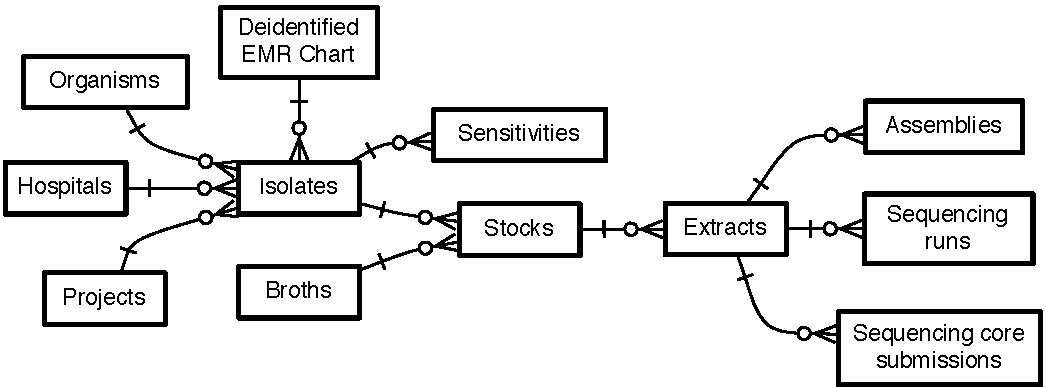
\includegraphics[width=\textwidth]{chap4/db-relations}               
  \caption[Entity-relationship diagram for the database underlying PathogenDB]{\textbf{Entity-relationship diagram for the database underlying PathogenDB,} using Information Engineering notation; see \textcite{Halpin2010}. Boxes represent tables of entities; single lines represent relationships, with arrowheads indicating the cardinality of each side of the relationship; crow’s foot arrowhead with circle represents “zero or more;” cross-stroke arrowhead represents “exactly one.”}
  \label{fig:pdb_relations}
\end{figure}
mirrors the workflow of banking and preparing isolates, with steps proceeding roughly left to right starting from ``Isolates''—i.e., isolates can associated with one or more derivative stocks once culturing and banking are performed, which will then be associated with one or more extracts, which are then submitted to the Genomics Core Facilty at Mount Sinai (``sequencing core submissions''). The returned outputs from Genomics Core are logged as ``sequencing runs'' and then eventually ``assemblies'' are created upon completion of the \pathogendbpipeline{} (see next section). Maintaining a database for each step of the process ensures that items are not lost along the way, and that the provenance of every downstream product can be traced backwards, which is crucial if contamination or mishandling are suspected.

\begin{sidewaysfigure}[hp]
  \sidewaysvspace
  \centering
  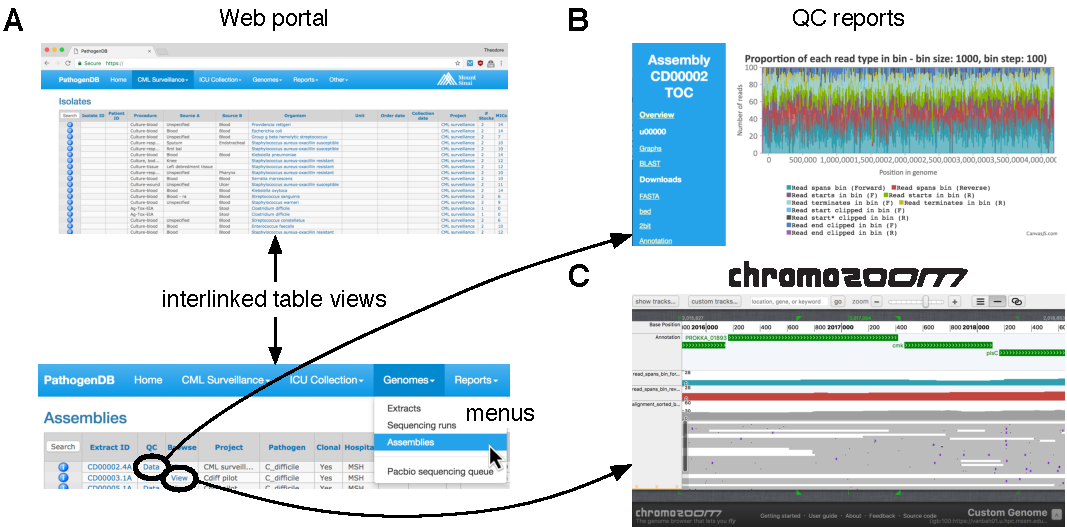
\includegraphics[width=\textwidth]{chap4/pdb-ui}               
  \fullwidthlabelcaption{fig:pdb_ui}{Overview of the web frontend for PathogenDB}{\textbf{Overview of the web frontend for PathogenDB.} A, the web portal permits quick access to basic views for all tables in the database, which can be searched, sorted, edited, and downloaded. At top, the Isolates table is shown, with certain potentially identifying information removed from the screenshot. At bottom, a zoomed view of the Assemblies table is shown, with the menu for switching between tables also shown. Links to special views (in B and C) are highlighted. B, sample quality control (QC) report for an assembly. Here, a graph of proportions of aligned reads that match various criteria is shown. Extreme fluctuations in these values can indicate assembly problems. C, ChromoZoom displaying a finished assembly, with annotated genes at top, two QC tracks in the center, and alignments of error corrected reads to the finished assembly at bottom. For more on ChromoZoom, see Chapter \ref{chap:chromozoom}.}
\end{sidewaysfigure}

PathogenDB provides a frontend that is based on phpMyEdit,\footnote{\url{http://www.phpmyedit.org/}} which is displayed in Figure \ref{fig:pdb_ui}. phpMyEdit allows for quick scaffolding of basic create-read-update-delete (CRUD) webpages for each of the tables in PathogenDB, which can be sorted, searched, edited, and downloaded by authorized members of the team. Authorization can be granted only to particular pages and views so that Bakel lab staff see only tables related to the isolate culturing and extraction workflow, while clinical coordinators instead see tables on patients due for sample collection and forms for sample submission.

Figure \ref{fig:pdb_ui}A shows a sample table view for the Isolates table, which tracks every biosample received by the Pathogen Surveillance Program. Isolates are associated with a Projects; if collected as part of routine operations, this is ``CML surveillance,'' but this field accommodates annotation of samples acquired from ad-hoc and outside investigations. Links at the far right of the table for Stocks and Minimum Inhibitory Concentrations (MICs) indicate that most Isolates are associated with two stocks and up to 14 measurements of antimicrobial susceptibility, which are extracted from Vitek (bioMérieux) results in the reports sent nightly by the EMR. Clicking on these links moves the user to a view of the corresponding entries in the related tables. On the Assemblies page, shown at the bottom of this panel, special views are provided for viewing outputs of the \pathogendbpipeline{} (after assembly and annotation are complete). The first of these is a quality control (QC) report (Figure \ref{fig:pdb_ui}B), which shows plots of the final contig layout and read statistics, which can be useful for assessing trustworthiness of the assembly and diagnosing reasons for failure to circularize or high fragmentation. The second of these is a link to a ChromoZoom visualization of the genome (Figure \ref{fig:pdb_ui}C, also see Chapter \ref{chap:chromozoom}).

\subsection{\pathogendbpipeline: Assembly and annotation from long reads}

Once read data are available from the Genomics Core, computational analysis can begin. To date, the Pathogen Surveillance Program has chosen to sequence essentially all isolates on the PacBio RS II (see Methods, Chapter \ref{chap:steno}). This sequencing platform comes with a manufacturer-maintained analysis toolkit called SMRT-Analysis\footnote[][-2.5cm]{\url{https://github.com/PacificBiosciences/SMRT-Analysis}} that we leverage for certain steps, which even includes a web interface (SMRT Portal), but we focus here on a fully automated solution.

\begin{figure*}[hb]
  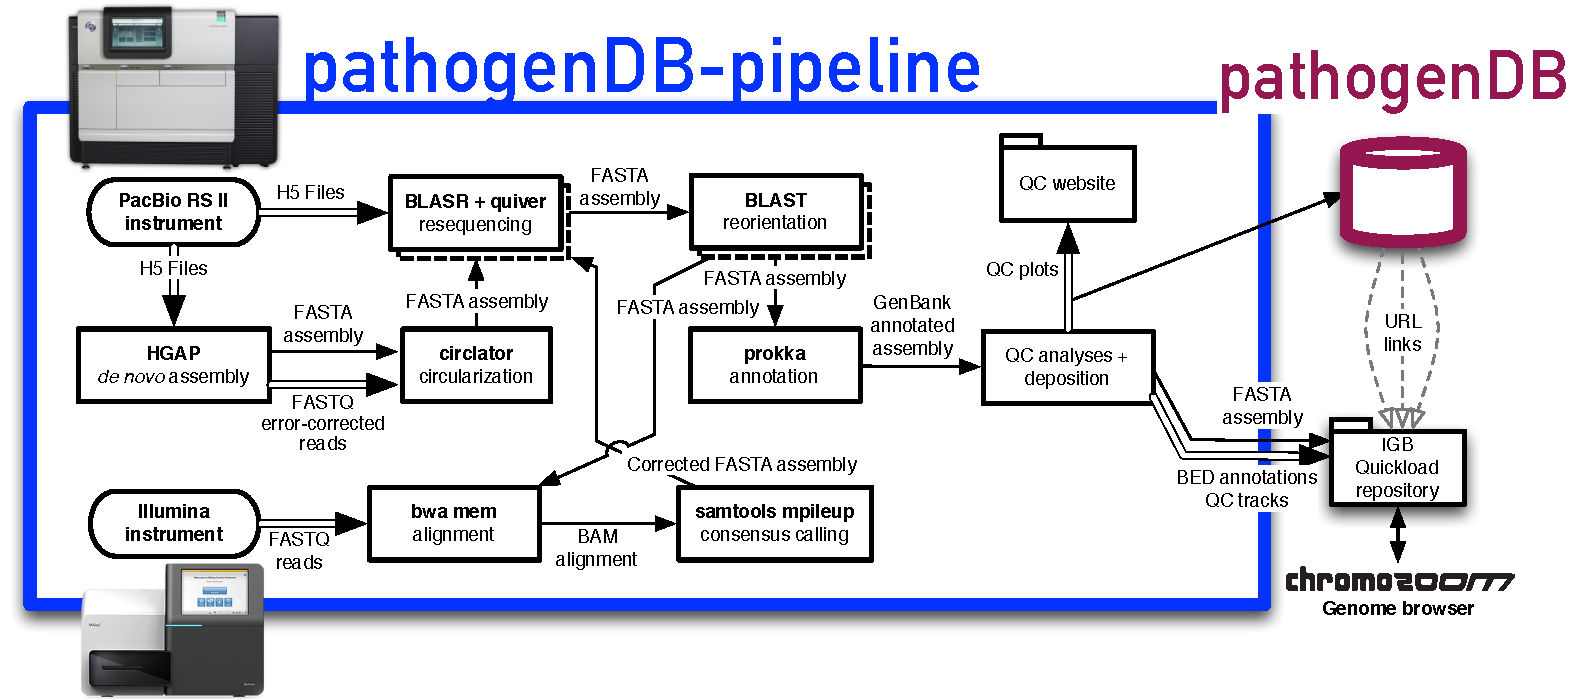
\includegraphics[width=\textwidth]{chap4/pdb-pipeline}               
  \caption[Outline of steps automated by \pathogendbpipeline]{\textbf{Outline of steps automated by \pathogendbpipeline.} Processes are depicted as boxes, with processes requiring potentially multiple runs indicated as a ``stack.'' An interim file format is depicted as a single arrow, and groups of files as doubled arrows. The pipeline concludes with deposition of a link to an IGB Quickload Directory for the completed assembly into PathogenDB.}
  \label{fig:pdb_pipeline}
  \setfloatalignment{b}
\end{figure*}

The chosen strategy for converting PacBio RS II reads into a final annotated assembly is outlined in Figure \ref{fig:pdb_pipeline}. Briefly, the H5 outputs of the instrument (which contains movies of the single molecule reads) are assembled \emph{de novo} using the Hierarchical Genome Assembly Process\autocite{Chin2013} (HGAP), which is included in SMRT-Analysis. This produces a draft assembly, but since HGAP cannot create circular contigs, a FASTA of this assembly and the FASTQs of error-corrected reads produced by HGAP are passed off to \texttt{circlator},\autocite{Hunt2015} a recently released tool that automates \emph{circularization} by using SPAdes\autocite{Bankevich2012} to re-assemble the error-corrected reads that overlapped the ends of contigs. This produces a new assembly that is then \emph{polished} over the circularized junctions by re-mapping raw reads using BLASR\autocite{Chaisson2012} and recalling the consensus with Quiver,\autocite{Chin2013} which reduces errors in these regions by re-incorporating read information that could not have aligned properly during the initial HGAP assembly. The polished assembly is then \emph{reoriented} back to the origin of replication (a convention for GenBank bacterial chromosome sequences) using a custom script\footnote{ \texttt{scripts/post\textunderscore quiver\textunderscore orient\textunderscore correct.py} in the \href{https://github.com/powerpak/pathogendb-pipeline/blob/master/scripts/post\textunderscore quiver\textunderscore orient\textunderscore correct.py}{GitHub repo}.} that performs a BLAST against \texttt{circlator}'s suggested origin point for each circular contig, which it decides based on a PROmer\autocite{Kurtz2004} search for \emph{dnaA} sequences.

The circularized, polished, and reoriented assembly is finally ready for annotation. Firstly, the contigs are renamed from the overly verbose HGAP and Quiver defaults. We use an in-house convention of starting all contig names with ``\texttt{u}'' (for ``unitig'', a term from Celera\footnote{See \url{http://wgs-assembler.sourceforge.net/wiki/index.php/Celera_Assembler_Terminology}}) followed by a five-digit unitig number originally assigned by HGAP. This is followed by three letters that flag for \underline{c}ircularization, \underline{r}eorientation, \underline{p}olishing, and an additional letter reserved for later use, with ``\texttt{x}'' indicating failure of that step. Another letter surrounded by underscores signals the hypothesized type of contig (\underline{c}hromosome, \underline{p}lasmid, \underline{m}erged, \underline{g}arbage, or \underline{o}ther).\footnote{We use the simple heuristic that any successfully circularized contig >1Mbp is a chromosome, and anything smaller is a plasmid. Merged and garbage contigs are the result of ambiguities during assembly. For more detail, see \href{https://github.com/powerpak/pathogendb-pipeline/blob/master/scripts/post\textunderscore circlator\textunderscore contig\textunderscore rename.py}{\texttt{scripts/post\textunderscore circlator\textunderscore contig\textunderscore rename.py}}.} Finally, the original SMRT-analysis job number set by the Genomics Core is appended. This renaming results in a contig ID like \verb|u00011crpx_p_023011|, indicating it is the 11th unitig, was \underline{c}ircularized, \underline{r}eoriented, and \underline{p}olished, is probably a \underline{p}lasmid, and came from sequencing job \#023011. These names are short enough for easy viewing in downstream tools like ChromoZoom, while retaining as much information as possible about the provenance and assembly status of the contig. Renamed contigs are finally annotated with \texttt{prokka},\autocite{Seemann2014} which detects putative coding regions and maps them to annotated gene names in UniProt.\autocite{Wasmuth2016} We then run a series of custom scripts to generate diagnostic files for the QC webpage (Figure \ref{fig:pdb_ui}B) and to convert the assembly and related tracks into an IGB Quickload Directory that can be loaded into ChromoZoom (Figure \ref{fig:pdb_ui}C).

\newthought{\pathogendbpipeline{}} is implemented as a \texttt{Rakefile}, which is written in Ruby and executed by \texttt{rake}, an analog of GNU \texttt{make}.\footnote{GNU \texttt{make} also inspired SnakeMake, a bioinformatics-focused build system for Python; see \textcite{Koster2012}.} GNU \texttt{make} was originally written as a build system for automating the generation of executables and other products from a program's source files. The advantage of a build system is that it encourages the explicit annotation of dependencies between interim files and tasks into the pipeline, thereby allowing for previous products of a partial build to be automatically re-used if their dependencies (source files) have not changed. From the user's perspective, another benefit is that only the desired final task in the pipeline needs to be specified, and \texttt{rake} can automatically figure out what preceding tasks are required to get to that point. For most runs, the sequence of tasks selected by \pathogendbpipeline{} is the following:

\begin{enumerate}[label=\arabic*.,noitemsep,labelindent=2em,leftmargin=!]
\item \verb|pull_down_raw_reads|
\item \verb|assemble_raw_reads|
\item \verb|run_circlator|
\item \verb|post_circlator|
\item \verb|resequence_assembly|
\item \verb|post_quiver_orient_correct|
\item \verb|prokka_annotate|
\item \verb|create_QC_webpage|
\item \verb|prokka_to_igb|
\end{enumerate}

which mostly correspond, unsurprisingly, to the boxes in Figure \ref{fig:pdb_pipeline}. Most of these tasks require at least one configuration option, such as the expected species or the destination for output. These are specified as environment variables during invocation, so to get to the final \verb|prokka_to_igb| step above, the user would run something like:

\begin{verbatim}
    $ rake OUT=scratch/out/ER05681 \
           SMRT_JOB_ID=023154 \
           STRAIN_NAME=ER05681 \
           SPECIES="Staphylococcus aureus" \
           prokka_to_igb
\end{verbatim}

If problems occur during assembly, the pipeline supports manual editing of the interim FASTA files, and then a flag (\texttt{CURATED=1}) can be set to signify that manual curation occurred and to therefore bypass circularization, reorientation, and contig renaming. There is also an optional branch (bottom entry point for Figure \ref{fig:pdb_pipeline}) that can incorporate Illumina short reads during assembly. Auxiliary sequencing on a short read platform can correct small errors that HGAP on PacBio reads will miss—typically indels in homopolymeric stretches. For this branch, \texttt{bwa}\autocite{Li2010b} is used to perform in-memory alignment against the circularized, reoriented, and polished assembly, and \texttt{samtools}\autocite{Li2009b} and \texttt{vcftools}\autocite{Danecek2011a} are used to call variants from the pileup and create a new FASTA consensus. These steps can in fact be repeated several times (crossover loop in Figure \ref{fig:pdb_pipeline}) to call a progressively more accurate consensus, although this repetition must currently be invoked manually.\footnote{A future version of the pipeline might attempt to re-run the steps until the consensus stabilizes.}

The modularity of siloing tasks in a \texttt{Rakefile} provided long-term advantages besides those mentioned previously. In our case, when we first created the pipeline in 2013, mature tools for some of the steps did not yet exist, e.g., \texttt{circlator} and \texttt{prokka} were not yet publicly available. Therefore, we used less efficient solutions, such as our own custom script for circularization and the RAST web service\autocite{Aziz2008} for annotation, as in Chapter \ref{chap:steno}. Once mature tools became available, it was relatively simple to swap them into the pipeline while preserving the old code under an \texttt{old:} namespace, indicating tasks that are deprecated. Because each task and its dependencies are relatively isolated, different members of the team can create slightly different versions of certain interim steps while still sharing all code in one common \texttt{Rakefile} pipeline. This was of course further reinforced by keeping all code under version control.\footnote{\url{https://github.com/powerpak/pathogendb-pipeline}}

\subsection{\pathogendbcomparison: Rapid comparative genomics}

\newthought{After deposition} of a complete annotated assembly's IGB Quickload Directory and corresponding record into the Assemblies table of PathogenDB, the next logical step of analysis is to compare all genomes for a given species (perhaps with some filtering by timeframe or location) to determine relatedness and the likelihood of transmissions. We implemented these analyses within the next module of our suite, called \pathogendbcomparison.

\begin{figure*}[htb]
  \centering
  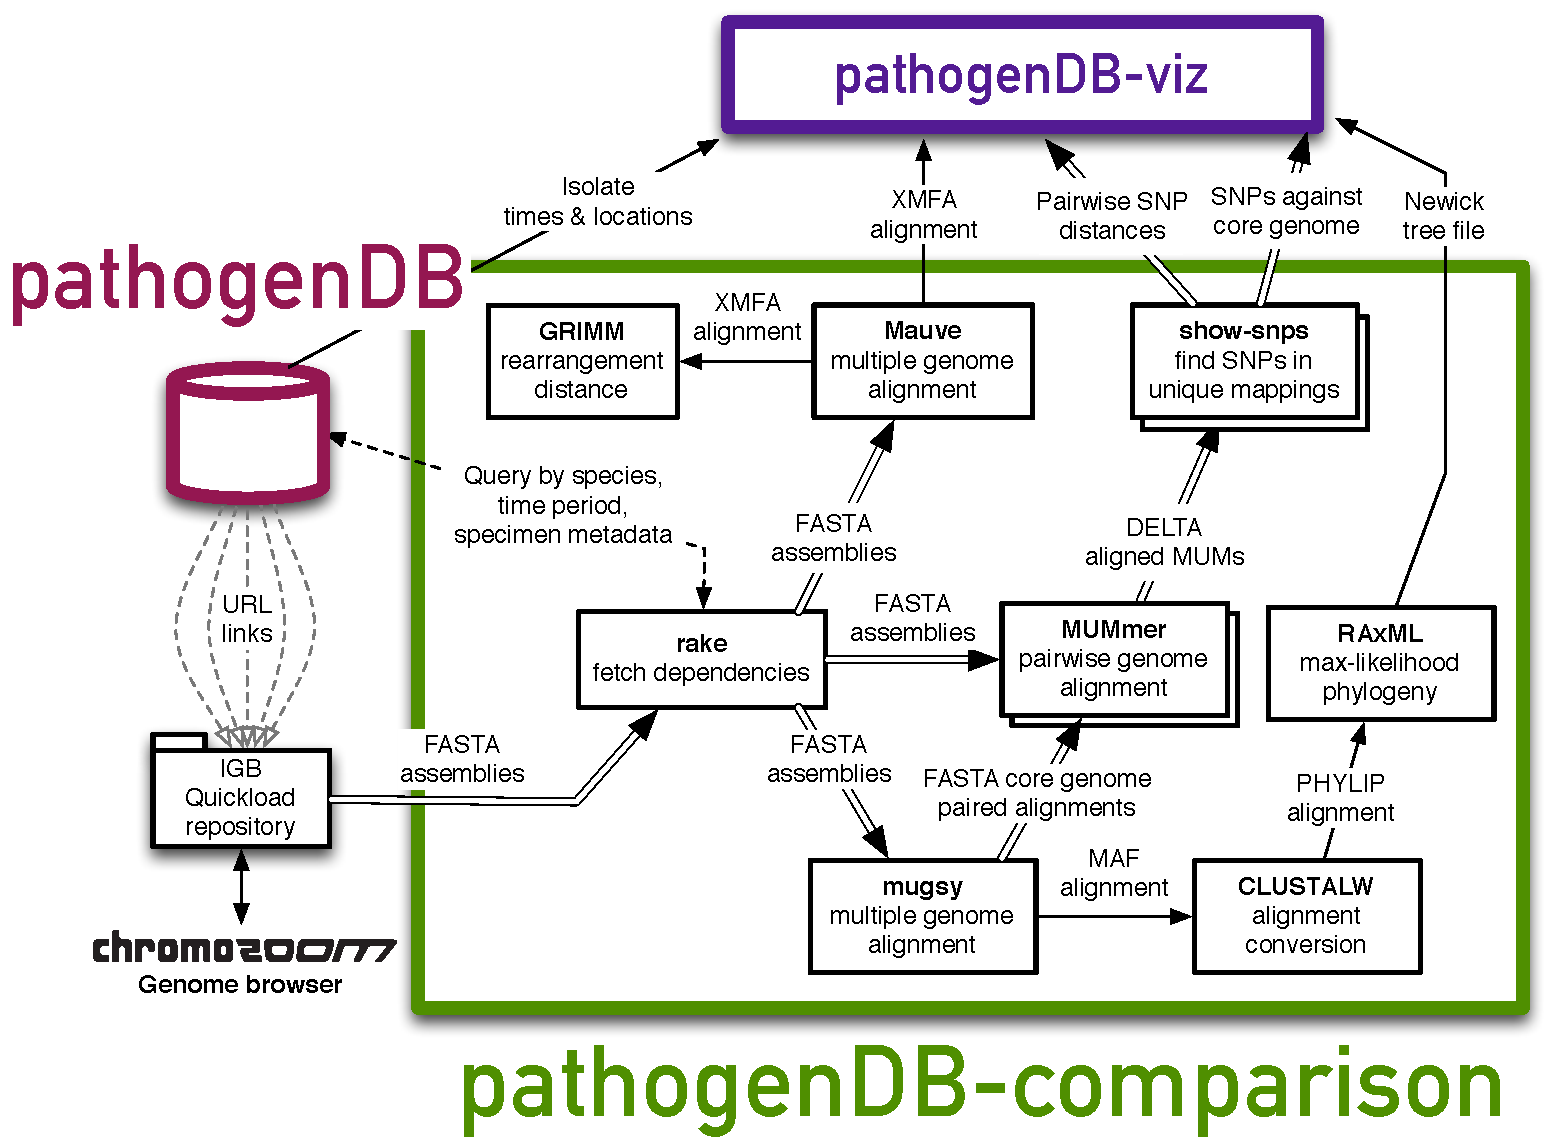
\includegraphics[width=0.8\textwidth]{chap4/pdb-comparison}               
  \caption[Outline of steps automated by \pathogendbcomparison]{\textbf{Outline of steps automated by \pathogendbcomparison.} Processes are depicted as boxes, with processes requiring potentially multiple runs indicated as a ``stack.'' An interim file format is depicted as a single arrow, and groups of files as doubled arrows. The pipeline concludes with various outputs being sent to \pathogendbviz for further visualization.}
  \label{fig:pdb_comparison}
\end{figure*}

Our implementation of workflows for this stage of analysis is outlined in Figure \ref{fig:pdb_comparison}. As emphasized previously, PathogenDB is considered the single source of ``truth'' from which all assemblies and metadata are queried before running an analysis; however, some of the tasks are generic enough to run on an arbitrary set of FASTA files without metadata. Like \pathogendbpipeline, \pathogendbcomparison{} is also implemented using \texttt{rake}, but its workflow is more branched. The three types of implemented analyses, reflected in Figure \ref{fig:pdb_comparison} by the three arrows emerging from the \texttt{rake} box and listed here with their corresponding \texttt{rake} task names, are:

\begin{enumerate}[label=\arabic*.,noitemsep,labelindent=2em,leftmargin=!]
\item \verb|mauve|: Mauve alignment, which highlights structural variants
\item \verb|snv|: Pairwise MUMmer single nucleotide variant (SNV) distances for heatmap visualization
\item \verb|mugsy|: Core genome alignment for a phylogeny with branch lengths scaled to SNV distances
\end{enumerate}

A Mauve alignment of \emph{S. maltophila} genomes was previously depicted in Figure \ref{fig:mauve} and is most useful for finding large insertions, deletions, translocations, and other recombinatorial events. Mauve performs alignments by using an anchoring heuristic to search for large areas of homology among subsets of the input genomes, which it terms local collinearity blocks (LCBs).\autocite{Darling2010} Our corresponding task simply wraps execution of \texttt{progressiveMauve}\autocite{Darling2010} and returns the XMFA alignment, since visualization is typically performed with the Mauve Java application. However, we also provide a task that can calculate pairwise rearrangement distances using GRIMM,\autocite{Tesler2002} which searches for the minimal number of inversion operations needed to transform one genome's sequence of LCBs into another genome's. Because inversion distance is algorithmically simple to calculate\autocite{Hannenhalli1999} but probably reflects evolutionary edit distances less accurately than newer models like double-cut and join (DCJ),\autocite{Lin2008} we have not yet made full use of these distances, but hope to eventually incorporate a wide array of structural variant edit distances into downstream analysis.\autocite{Hilker2012}

MUMmer is a versatile software suite for fast pairwise genome alignment that finds maximally exact matches (formerly maximal unique matches, hence MUM) using a suffix tree algorithm that can run in linear time.\autocite{Kurtz2004} Although it is excellent for finding subsequences of one genome that are within a certain edit distance of all locations on another genome, because of the strict edit distance threshold, it is less suited for finding large rearrangements compared to Mauve. However, it is very well suited for quickly calling SNVs between two genomes, as long as the SNVs are not so closely spaced as to elude a maximally exact match for the surrounding region (which should occur only extremely rarely). For this task, we use the \texttt{show-snps} tool within MUMmer to call SNVs between all pairs of input genomes, which produces a distance matrix that can be visualized with \pathogendbviz{} (see Results).

The same strategy is also used to rescale branches for our phylogenetic analysis, which we perform by creating a core genome alignment with \texttt{mugsy},\autocite{Angiuoli2011a} a multiple genome aligner that internally combines MUMmer and its own algorithm for finding LCBs.\footnote{Recently, the Harvest suite was released for core genome alignment, which scales better to thousands of genomes than \texttt{mugsy}, and it even includes its own visualization tool, \texttt{gingr}. We are currently in the process of incorporating these tools into our pipeline. For more, see \textcite{Treangen2014}} The core genome alignment in MAF format is converted to PHYLIP format with CLUSTALW,\autocite{Sievers2011} and then this alignment undergoes maximum-likelihood phylogenetic inference via RAxML.\autocite{Stamatakis2005} Since the outputted tree (in Newick format) initially has distances in units of time under the RAxML evolutionary model, which is more opaque than SNV distance, the tree's branches are rescaled by recalculating SNV distance using the aforementioned \texttt{show-snps} method on all adjoining nodes, including the ancestral states imputed by RAxML. Phylograms of these trees with overlaid SNV distances (as in Figure \ref{fig:steno_phylo}) can be plotted to PDFs using an included \verb|mugsy_plot| task that wraps the \texttt{ape} R package.

Although maximum likelihood phylogenetic analysis is a standard component of molecular epidemiology and typically the centerpiece of most published investigations of outbreaks using NGS,\autocite{Azarian2015,Eyre2012,Joensen2014,Casali2016} it may in fact be overkill for answering the simpler day-to-day question of ``are any new isolates closely related to the previously sequenced isolates?'' By design, it requires a core genome alignment for all of the genomes that one wishes to include in the tree. Although every multiple sequence aligner uses heuristics to save time, multiple sequence alignment has a fundamental algorithmic complexity of $O(g^n)$ under the usual dynamic programming approaches,\autocite{Just2004} where $g$ is the average length of a genome and $n$ is the number of genomes—i.e., exponential to the number of genomes. Even though tools for core genome alignment continue to get smarter and faster about subverting this complexity,\autocite{Treangen2014} given the fundamental difficulties in scaling that problem, we anticipate that pairwise distance matrices will be a suitable alternative for outbreak detection as databases of thousands of assembled sequences become commonplace. Creating a distance matrix is guaranteed to be $O(n^2)$ in the most naive approach,\footnote{And this is how it is currently implemented; precalculating the MLST for all isolates and only allowing within-MLST comparisons would be a simple first optimization.} with each pairwise comparison being $O(g)$ by use of \texttt{show-snps}. Furthermore, adding one new assembled isolate does not require recalculating everything as in multiple sequence alignment, but we can instead add one row and column to the existing matrix in $O(2n)$ time. For these reasons we provide the \verb|snv| task in conjunction with \verb|mugsy|, and we rely on the distance matrices for analyses on >100 genomes, as presented later in the Results.

\subsection{\pathogendbviz}

\newthought{Visualization} is finally performed with the \pathogendbviz{} toolkit. The interface, which has a heatmap layout and a geospatial layout, will be presented in the Results in Figures \ref{fig:pdb_heatmap_saureus}-\ref{fig:pdb_geospatial_cdiff}. \pathogendbviz{} reads data from JSON files containing genetic distances and isolate metadata as prepared by \pathogendbcomparison{}'s \verb|heatmap| task, and displays it in a HTML5 interface that draws data dynamically to scalable vector graphics (SVG) using the d3.js Javascript library.\footnote{\url{https://d3js.org/}} \pathogendbviz{} is currently implemented as a single PHP page that loads all data via Asynchronous Javascript and XML (AJAX).\autocite{Paulson2005} Given that all data is drawn on the client side, it attempts to maximize the control the user has over the selection of isolates to displayed and how the comparison is presented. Agglomerative hierarchical clustering is performed in the browser using the \texttt{ml-hclust}\footnote{\url{https://www.npmjs.com/package/ml-hclust}} node.js package, using single linkage to emphasize the ``chaining'' of closely related genomes into clusters. The heatmap.js\footnote{\url{https://www.patrick-wied.at/static/heatmapjs/}} library is used to draw density plots of epidemiological incidence in the geospatial layout. Sequenced isolates are displayed in the geospatial layout as a live-updating force-directed network using \texttt{d3.forceSimulation}, with a strong force keeping nodes from colliding, a moderate force pulling nodes toward the position of specimen collection, and a very weak spring force along the edges (which represent the putative transmissions under the selected SNV threshold).

\subsection{Availability}

Source code for \pathogendbpipeline, \pathogendbcomparison, and \pathogendbviz{} is publicly available from GitHub at:

\begin{enumerate}[label=\arabic*.,noitemsep,labelindent=2em,leftmargin=!]
\item \url{https://github.com/powerpak/pathogendb-pipeline}
\item \url{https://github.com/powerpak/pathogendb-comparison}
\item \url{https://github.com/powerpak/pathogendb-viz}
\end{enumerate}

The code in each repository is still under active development to suit the operational needs of the Pathogen Surveillance Program. The software is currently configured for execution on Mount Sinai's high performance computing environment (Minerva), but we will adapt it for simple installation on vanilla Linux distributions and provide machine images suitable for common cloud computing environments once we are ready to promote usage by other groups.

\section{Results and Discussion}

\subsection{Assembly quality}

As of April 2017, \pathogendbpipeline{} has been used to assemble and annotate 593 genomes from 7 species. General statistics on assemblies produced by the pipeline are presented in Table \ref{tab:pathogendb_assemblies}. Most of the isolates assembled so far are \emph{Staphylococcus aureus} and \emph{Clostridium difficile} strains. About three quarters of the assembled \emph{S. aureus} isolates were methicillin-resistant (MRSA). A few other rarer species have also been assembled.\footnote{Note that the \emph{S. maltophilia} isolates from Chapter \ref{chap:steno} predate PathogenDB and therefore are not included in Table \ref{tab:pathogendb_assemblies}.} 164 assemblies underwent manual curation during the development of the pipeline and are excluded from statistics on assembly quality.

\begin{table}[htb]
  \centering
\small
\begin{tabular}{l l}
  \toprule
  Characteristic &
  Assemblies (\%), \emph{N}=593\\
  \midrule
  Species
  \\
  \-\tabindent \emph{Clostridium difficile} &
  221 (37.3)
  \\
  \-\tabindent \emph{Staphylococcus aureus}
  \\
  \-\tabindent\tabindent Methicillin-resistant &
  262 (44.3)
  \\
  \-\tabindent\tabindent Methicillin-resistant &
  90 (15.2)
  \\
  \-\tabindent \emph{Clostridium innocuum} &
  4 (0.7)
  \\
  \-\tabindent \emph{Enterococcus faecium} &
  4 (0.7)
  \\
  \-\tabindent Other &
  7 (1.1)
  \\
  \\
  Assembly quality (uncurated assemblies only) &
  Assemblies (\%), \emph{N}=429
  \\
  \midrule
  \-\tabindent \emph{N50} > 1Mbp &
  412 (96.0)
  \\
  \-\tabindent Circular chromosome$^a$ &
  303 (70.6)
  \\
  \-\tabindent Largest contig size
  \\
  \-\tabindent\tabindent ≥1Mbp &
  418 (97.4)
  \\
  \-\tabindent\tabindent ≥100kbp, <1Mbp &
  8 (1.9)
  \\
  \-\tabindent\tabindent <100kbp &
  3 (0.7)
  \\
  \-\tabindent Number of contigs
  \\
  \-\tabindent\tabindent 1 &
  102 (23.8)
  \\
  \-\tabindent\tabindent 2 &
  110 (25.6)
  \\
  \-\tabindent\tabindent 3 &
  71 (16.6)
  \\
  \-\tabindent\tabindent 4 &
  40 (9.3)
  \\
  \-\tabindent\tabindent ≥5 &
  84 (19.6)
  \\
  \bottomrule
\end{tabular}
  \caption[Statistics on assemblies generated by \pathogendbpipeline{} since 2013]{\textbf{Statistics on assemblies generated by \pathogendbpipeline{} since 2013.} $^a$Any contig ≥1Mbp that circularized was considered a chromosome. Abbreviations: N50, shortest contig length above which 50\% of the genome is included; Mbp, 1 million base pairs; kbp, 1 thousand base pairs.
}
  \label{tab:pathogendb_assemblies}
\end{table}

Without any curation (manual fixes), \pathogendbpipeline{} is able to completely assemble most of the sequenced isolates, with >70\% featuring a circular main chromosome. The \emph{N50}, defined as the shortest contig at which it and all larger contigs would include 50\% of the genome, was ≥1Mbp for 96.0\% of uncurated genomes. 80.4\% of completed assemblies contained four or fewer contigs, i.e., one chromosome (either closed or unclosed) and up to three plasmids or unassembled fragments. By these metrics, \pathogendbpipeline{} is clearly able to produce many high-quality \emph{de novo} assemblies without human intervention.

\subsection{Computational benchmarks for \pathogendbpipeline}

\begin{figure*}[htb]
  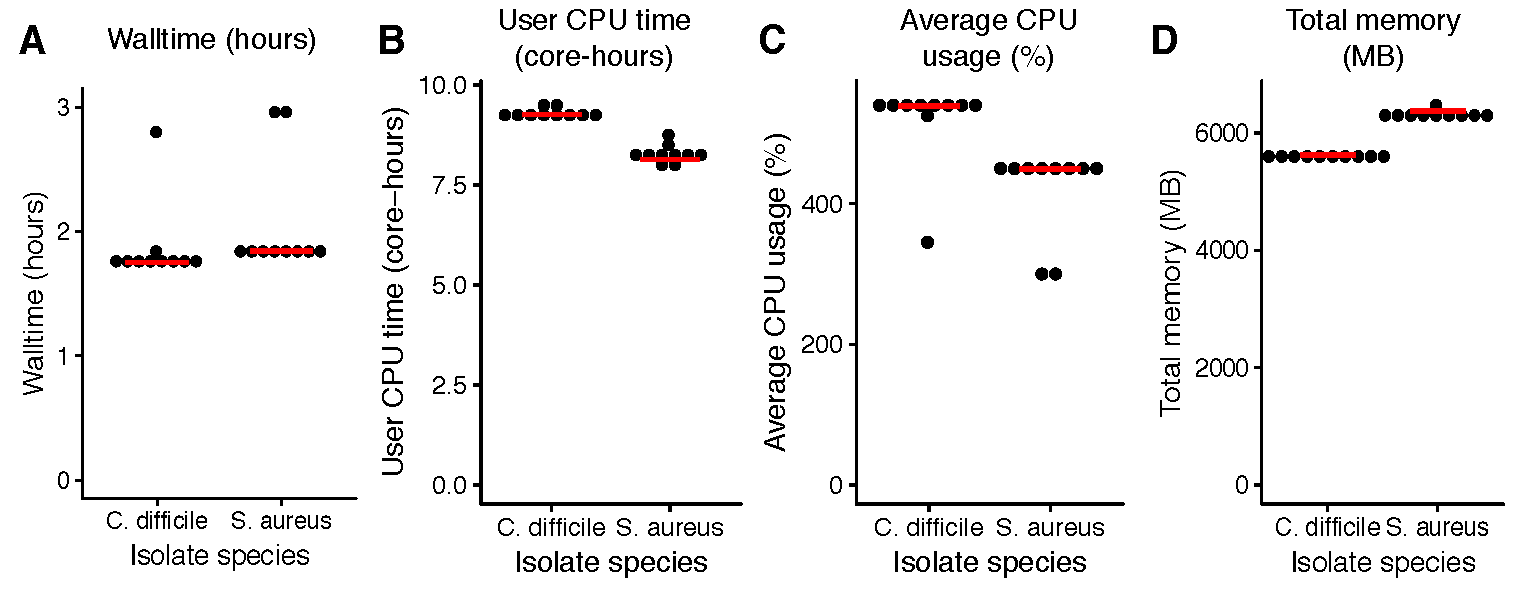
\includegraphics[width=\textwidth]{chap4/pdb-benchmark}               
  \caption[Boxplots of computational benchmarks for \pathogendbpipeline]{\textbf{Boxplots of computational benchmarks for \pathogendbpipeline{} on a \emph{S. aureus} and a \emph{C. difficile} isolate.} For each isolate, measurements were collected from 10 end-to-end serial runs of the pipeline, starting at raw read data and ending at the \texttt{prokka\textunderscore to\textunderscore igb} task, using a single server with a 12-core Intel Xeon(R) 2.5GHz E5-2680 CPU and 128GB of RAM.}
  \label{fig:pdb_benchmark}
\end{figure*}

Although over the past four years of development its end-to-end time has improved, \pathogendbpipeline{} is still by far the most computationally intensive module within the PathogenDB suite. The majority of the cost is accrued during the \emph{de novo} assembly and polishing steps, which require stepping through all read data for each sequenced isolate, which commonly exceeds 1Gbp per isolate. In Figure \ref{fig:pdb_benchmark} we provide benchmarks for the impact of \pathogendbpipeline{} on overall turnaround time for an end-to-end analysis and the corresponding computational cost. We performed 10 serial end-to-end runs of the pipeline starting from raw read data for one \emph{S. aureus} isolate and one \emph{C. difficile} isolate on a 12-core Intel Xeon(R) 2.5GHz E5-2680 server with 128GB of RAM. Most of the runs produced nearly identical benchmarks, so the interquartile ranges in Figure \ref{fig:pdb_benchmark} are very narrow. The median walltime (which measures real-world start to end time) was under two hours, with none of the runs exceeding three hours (Figure \ref{fig:pdb_benchmark}A). The jobs benefited from multicore usage, as the median user CPU time in core-hours exceeded the walltime by a factor of 4-5× (Figure \ref{fig:pdb_benchmark}B), and this is confirmed by checking average CPU usage, which is normalized against a single core and stayed mostly in the 400-600\% range (Figure \ref{fig:pdb_benchmark}C). Although HGAP, BLASR, and Quiver are memory-intensive steps, the total memory used did not exceed 7GB for any of the runs (Figure \ref{fig:pdb_benchmark}D).

\subsection{\pathogendbviz{} characterizes local outbreaks of \emph{S. aureus}}

After comparing a large number of same-species isolates with \pathogendbcomparison{}, the analyses can be presented to clinicians in an interactive visualization using \pathogendbviz. Figure \ref{fig:pdb_heatmap_saureus} displays the interface of \pathogendbviz{} for a heatmap visualization of all \emph{S. aureus} isolates that clustered with at least one other patient's isolate(s) at a SNV threshold of ≤10 SNVs. The software provides a web interface with many controls for quickly ``drilling down'' to the time range and isolates of interest. We now briefly tour this interface.

\begin{sidewaysfigure}[hp]
  \sidewaysvspace
  \centering
  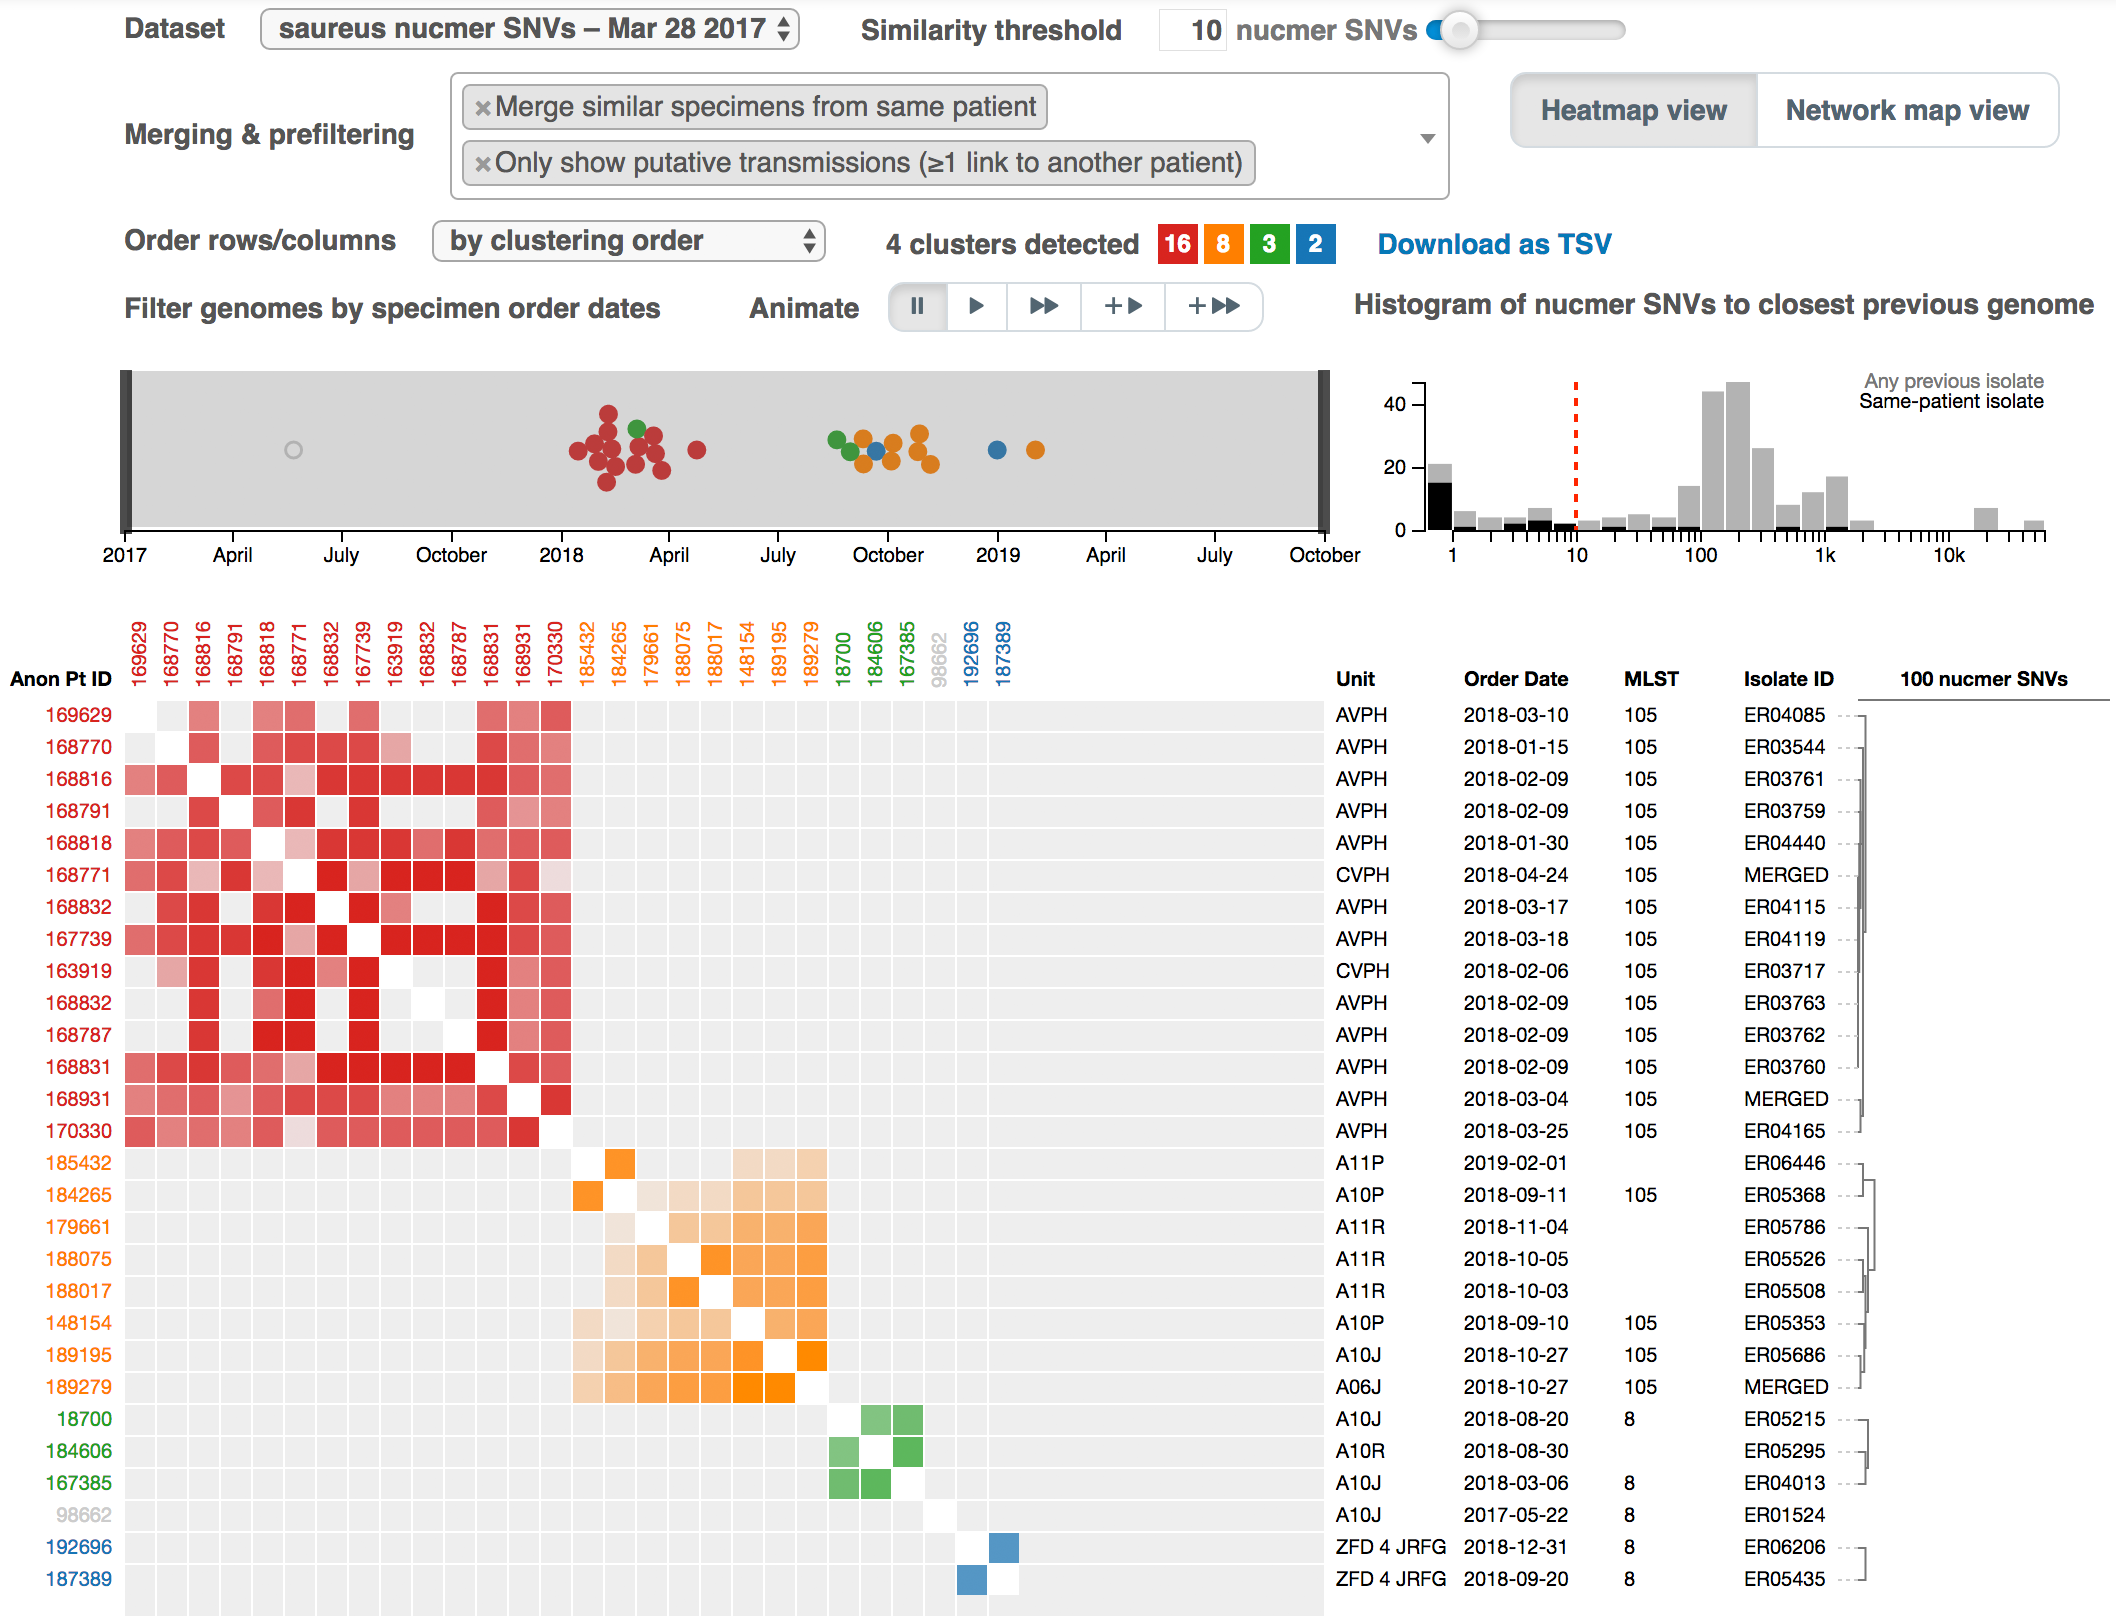
\includegraphics[width=0.85\textwidth]{chap4/pdb-heatmap-saureus}               
  \fullwidthlabelcaption{fig:pdb_heatmap_saureus}{\pathogendbviz{} heatmap visualization for all putatively transmitted \emph{S. aureus} isolates, based on NGS}{\textbf{\pathogendbviz{} heatmap visualization for all putatively transmitted \emph{S. aureus} isolates, based on NGS.} Note that dates have been shifted into the future and unit names have been obfuscated to reduce the disclosure of potentially identifying information. At top, user controls allow selection of the dataset, SNV threshold, merging and prefiltering of isolates, and ordering of the diagram. A horizontal beeswarm shows the distribution of isolates over collection times, which the user can ``brush'' to select specific time ranges. At adjacent right, a histogram of SNV distances between each genome and its closest previous neighbor helps inform what a reasonable SNV threshold might be; in black, isolates from the same patient (which are expected to be related); in gray, isolates from any previous patient. At bottom left, a clustered heatmap depicts distances between isolates that exceed the SNV threshold as the large colored blocks along the diagonal. At bottom right, a hierarchical clustering shows SNV distances between rows in the heatmap.}
\end{sidewaysfigure}

At top left, the user can select from analyses that were generated by the \verb|heatmap| task of \pathogendbcomparison. The top right has a slider used to set a threshold in SNVs for considering two isolates to be related enough for putative transmission. While previous studies suggest using a very low threshold, e.g., 2-3 SNVs for \emph{C. difficile} isolates collected within one year,\autocite{Eyre2013,Price2014,Eyre2012} these studies used short-read sequencing and alignment-based methods, which miss SNVs in regions that can't align to the chosen reference—particularly structural variants, plasmids, and long repeats. 

To justify a selected SNV threshold for a particular dataset, we provide a built-in analysis similar to what is presented in recent studies\footnote{See Figure 1A of \textcite{Eyre2013}.} as the histogram in the top right of the interface. This histogram shows the distribution of SNV distances from every genome to its closest (by SNV distance) neighbor among chronologically previous isolates, comparing the distributions for same-patient isolates (black) and different-patient isolates (gray). Actual transmissions should be reflected as a gray peak toward the left of the diagram (small distances), while the natural diversity of \emph{S. aureus} in the community creates a separate peak toward the center. Indeed, in our data, we see a clear bimodal distribution (Figure \ref{fig:pdb_heatmap_saureus}). Also, as same-patient isolates are expected to be share lineage, the left-side black peak serves as the ``positive control'' for distances that are representative of clonality in our data (and therefore would also imply transmission for different patient isolates). Based on the overlapping left-side peaks and the midpoint between the two gray peaks, a cutoff of ~10 SNVs appears reasonable for the depicted 2.7 year period to define continuity of lineage. This is consistent with the 5-10 SNV per year average mutation rate observed in recent NGS surveys of hospital-associated \emph{S. aureus}.\autocite{Price2014,Harris2013}

The user can specify merging and prefiltering options for isolates at the top left. The ``merge similar specimens from the same patient'' option is particularly useful for condensing the display, as it collapses all same-patient isolates under the SNV threshold into single datapoints.\footnote{Resampling is common in our dataset since some patients get standing orders for daily cultures and the Pathogen Surveillance Program receives all positive \emph{S. aureus} culture specimens.} This allows the user to focus on only the links between different-patient isolates. Similarly, the option to ``only show putative transmissions'' hides all isolates with no links to a different-patient isolate under the SNV threshold. What remains, in effect, are only the sequenced patient isolates involved in putative transmission events.

\pathogendbviz{} automatically performs clustering of the isolates that match the criteria. In Figure \ref{fig:pdb_heatmap_saureus}, over the 2.7 year period we see that four clusters were detected, with sizes of 16, 8, 3, and 2 patients. One of these clusters (red) was already known to infection control staff and resulted in the shutdown and deep cleaning of the involved hospital unit. The timeline beeswarm plot shows that all of these isolates fell within a roughly four month span, and the end of this span is when the cleaning occurred; thankfully, no new isolates related to this cluster have been detected since. The 8 patient cluster (orange), which spans a more recent interval of six months, was not known to infection control before sequencing occured, and in fact was discovered by use of this visualization.

The main area of the visualization (bottom left) shows a clustered heatmap of distances between the isolates that matched the filtering criteria. Each patient is both a row and a column, and a link between two patients underneath the SNV threshold results in a colored box. (Although not shown in Figure \ref{fig:pdb_heatmap_saureus}, these boxes can be clicked to reveal more detailed information about each patient isolate with links to corresponding records in PathogenDB.) Almost all isolates within a cluster should be related to each other underneath the SNV threshold, which results in large colored squares along the diagonal. The presence and size of these squares are an easy way for infection control officers viewing the data to judge how many ``clusters'' of transmission appear to be present in the time interval and the level of evidence for the coherence of a cluster. Pairwise MUMmer comparisons can result in spurious SNV calls in certain hypervariable regions (e.g., phage elements), which artificially inflates SNV distances and results in ``holes'' in the square (as in the red cluster).

The hierarchical clustering distances are shown as a more familiar tree at the bottom right of the visualization, along with metadata for each isolate like order date, MLST, and unit of collection. In this case, the metadata reveal that the red cluster was concentrated in a single unit (which is how infection control became aware of it via epidemiological data alone). The 8-patient orange cluster, however, is spread across multiple units.

\begin{sidewaysfigure}[hp]
  \sidewaysvspace
  \centering
  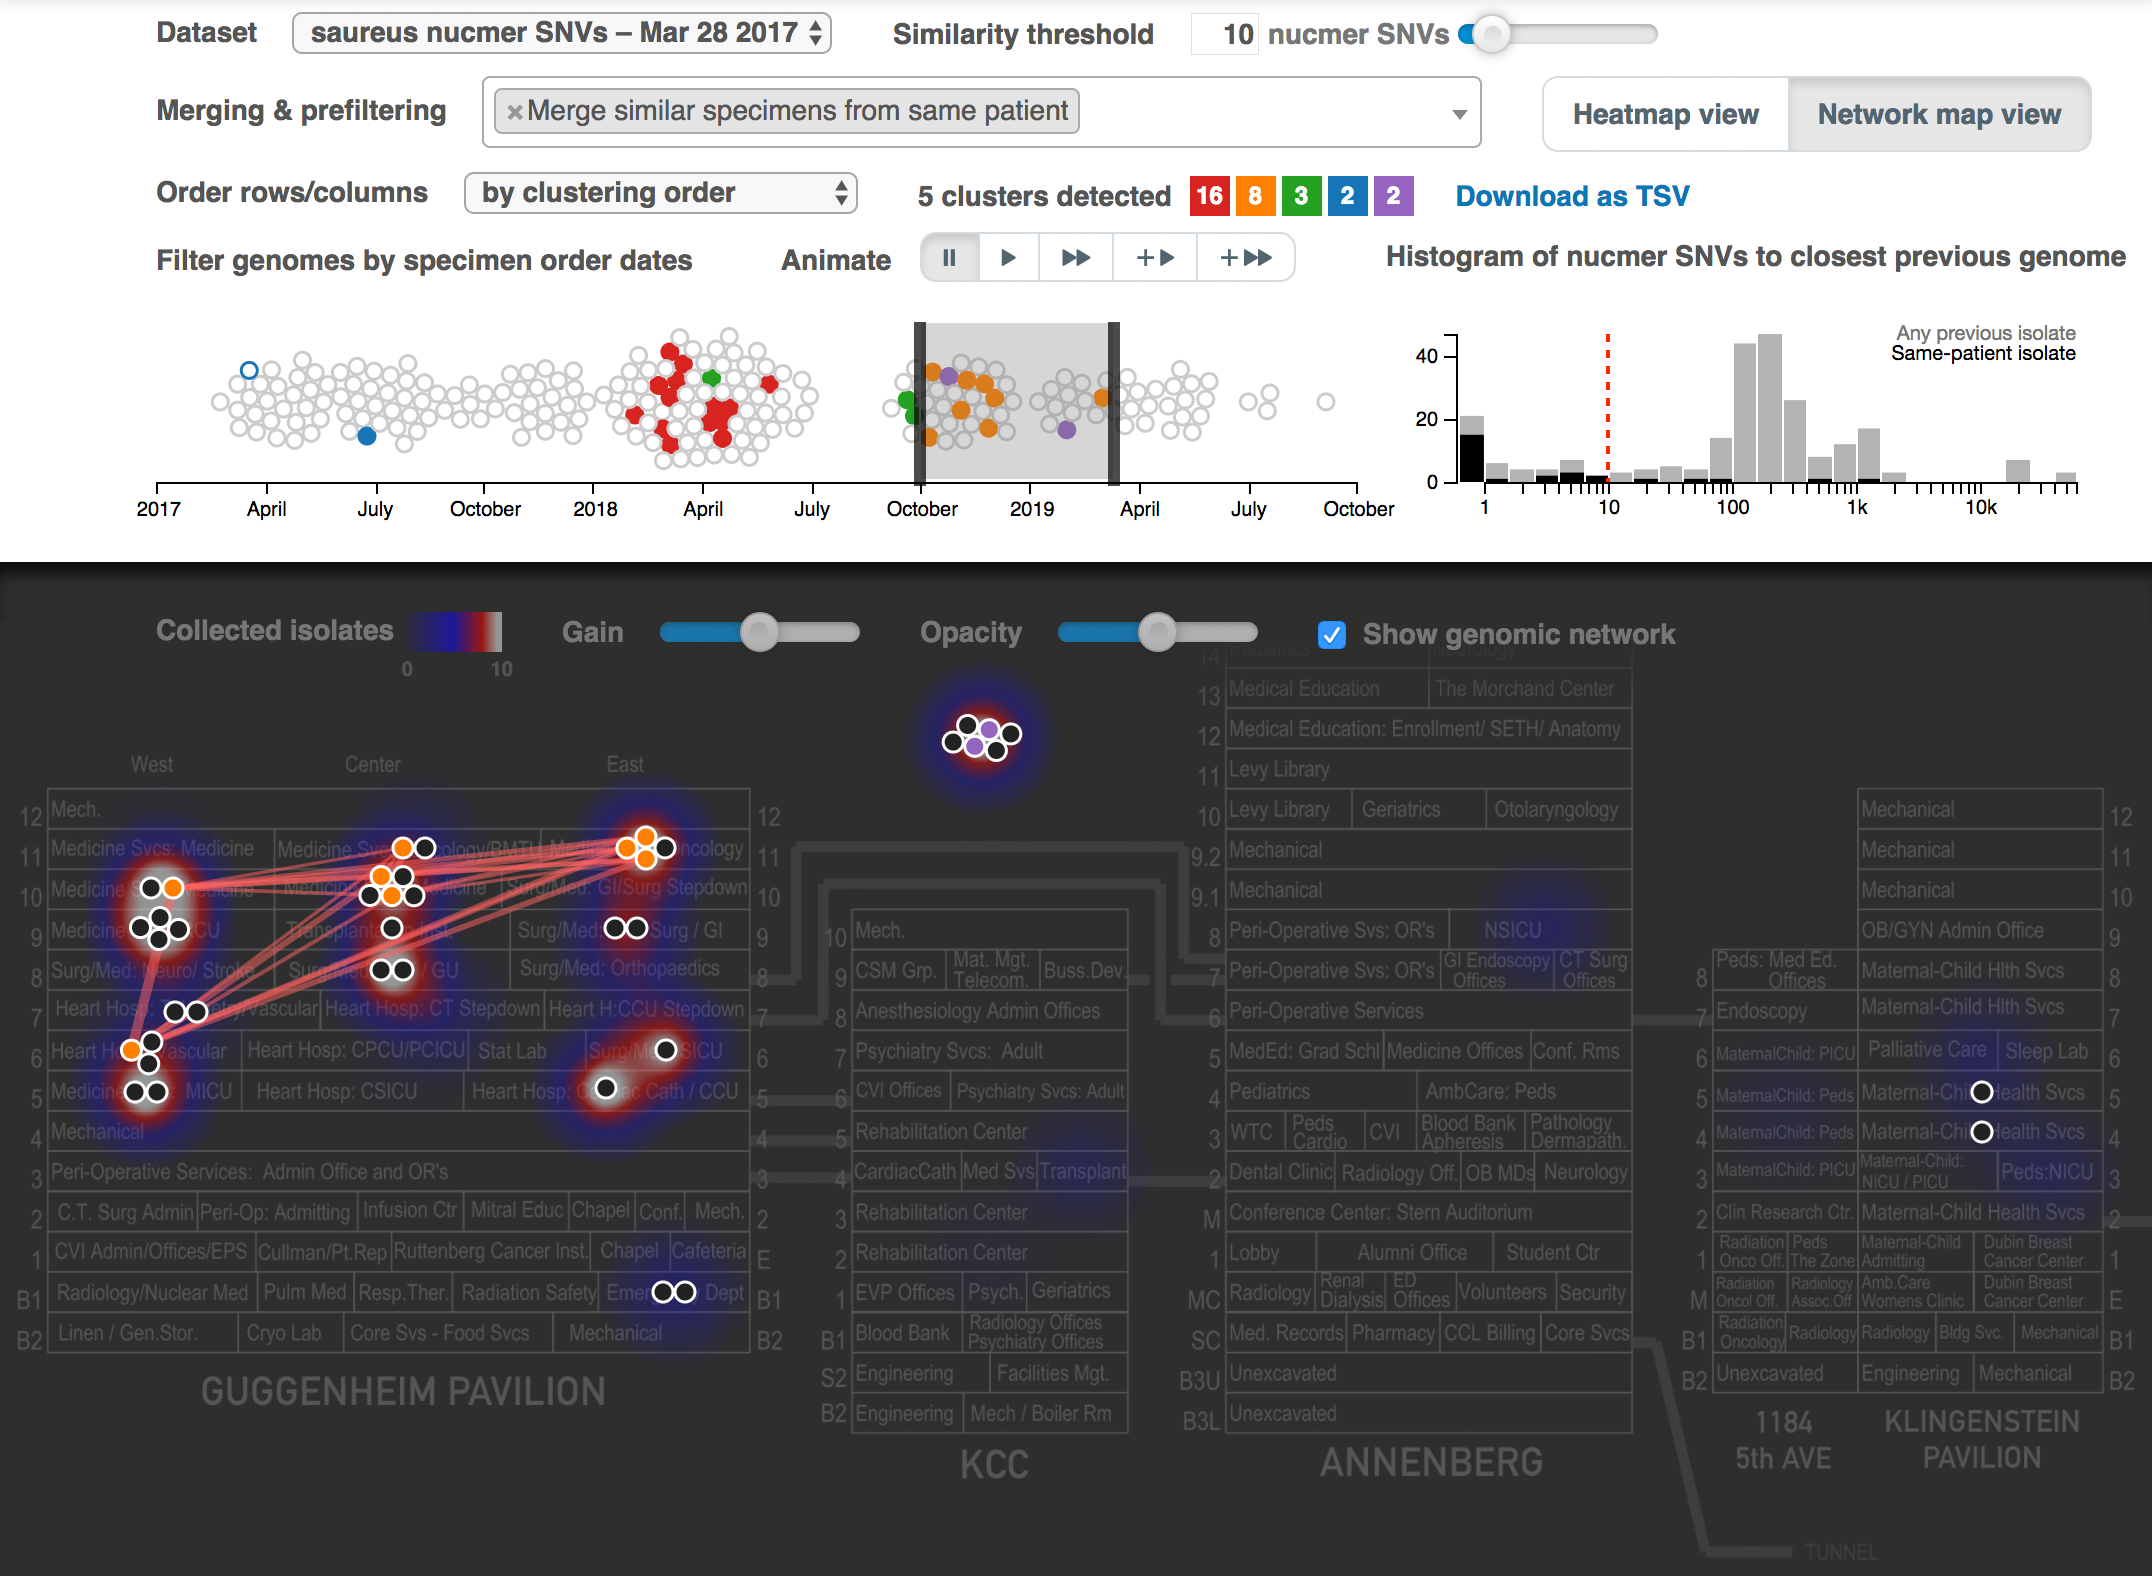
\includegraphics[width=0.9\textwidth]{chap4/pdb-geospatial-saureus}               
  \fullwidthlabelcaption{fig:pdb_geospatial_saureus}{\pathogendbviz{} geospatial visualization for an NGS-confirmed cluster of \emph{S. aureus} isolates}{\textbf{\pathogendbviz{} geospatial visualization for an NGS-confirmed cluster of \emph{S. aureus} isolates.} Note that dates have been shifted into the future to reduce the disclosure of potentially identifying information. The top of the interface is as in Figure \ref{fig:pdb_heatmap_saureus}. At bottom, node-link diagram of putative transmissions, with circles representing sequenced isolates in the selected time range (see timeline beeswarm plot) and red lines connecting isolates underneath the chosen SNV threshold (here, 10 SNVs). Nodes are placed on top of the hospital unit (light gray stacking diagram, vertical axis corresponds to floor level) from which the isolate was collected. The density plot underneath nodes represents the overall frequency of positive cultures at each location of the hospital.}
\end{sidewaysfigure}

\newthought{A spatial layout} can be useful to visualize isolates and their links in relationship to hospital locations, and is provided as an alternative view by \pathogendbviz{} (Figure \ref{fig:pdb_geospatial_saureus}). This interface, which is accessed by toggling the ``Network map view'' button in the upper right corner, has been focused on only the isolates in the time range of the orange cluster, although we now include unrelated isolates as well (note that the beeswarm timeline contains new light gray circles, which are the isolates that were not involved in any putative transmissions). In this view, the isolates are depicted as dots on top of a stacking layout of Mount Sinai's hospital campus, which has several different buildings (see the Guggenheim, KCC, and Annenberg labels at bottom). The floors are laid out vertically in this diagram, and connections between them (like sky bridges) are depicted as thick lines. (The isolates hovering over KCC were sent from Mount Sinai Queens.) Dots are colored by the cluster they were in, and transmissions between patients according to the SNV threshold are drawn as red lines. This diagram makes it apparent that the patients in the orange cluster were spread across the upper floors of the Guggenheim building, with at most three patients sharing a unit. The spatial network layout also includes a density plot (the fuzzy clouds underneath the points) that depicts all collected isolates in PathogenDB, including those not yet sequenced. Therefore, the density plot can reveal parts of the hospital that had many cases of the HAI, but have been undersampled by the NGS data, and could merit follow-up sequencing of the banked isolates. In the case of Figure \ref{fig:pdb_geospatial_saureus}, there are no clouds without dots, meaning that all ``hot spots'' for \emph{S. aureus} in the hospital during this time interval were at least partially captured in the NGS data.

\subsection{\pathogendbviz{} identifies local diversity and transmissions of \emph{C. difficile}}

\begin{sidewaysfigure}[hp]
  \sidewaysvspace
  \centering
  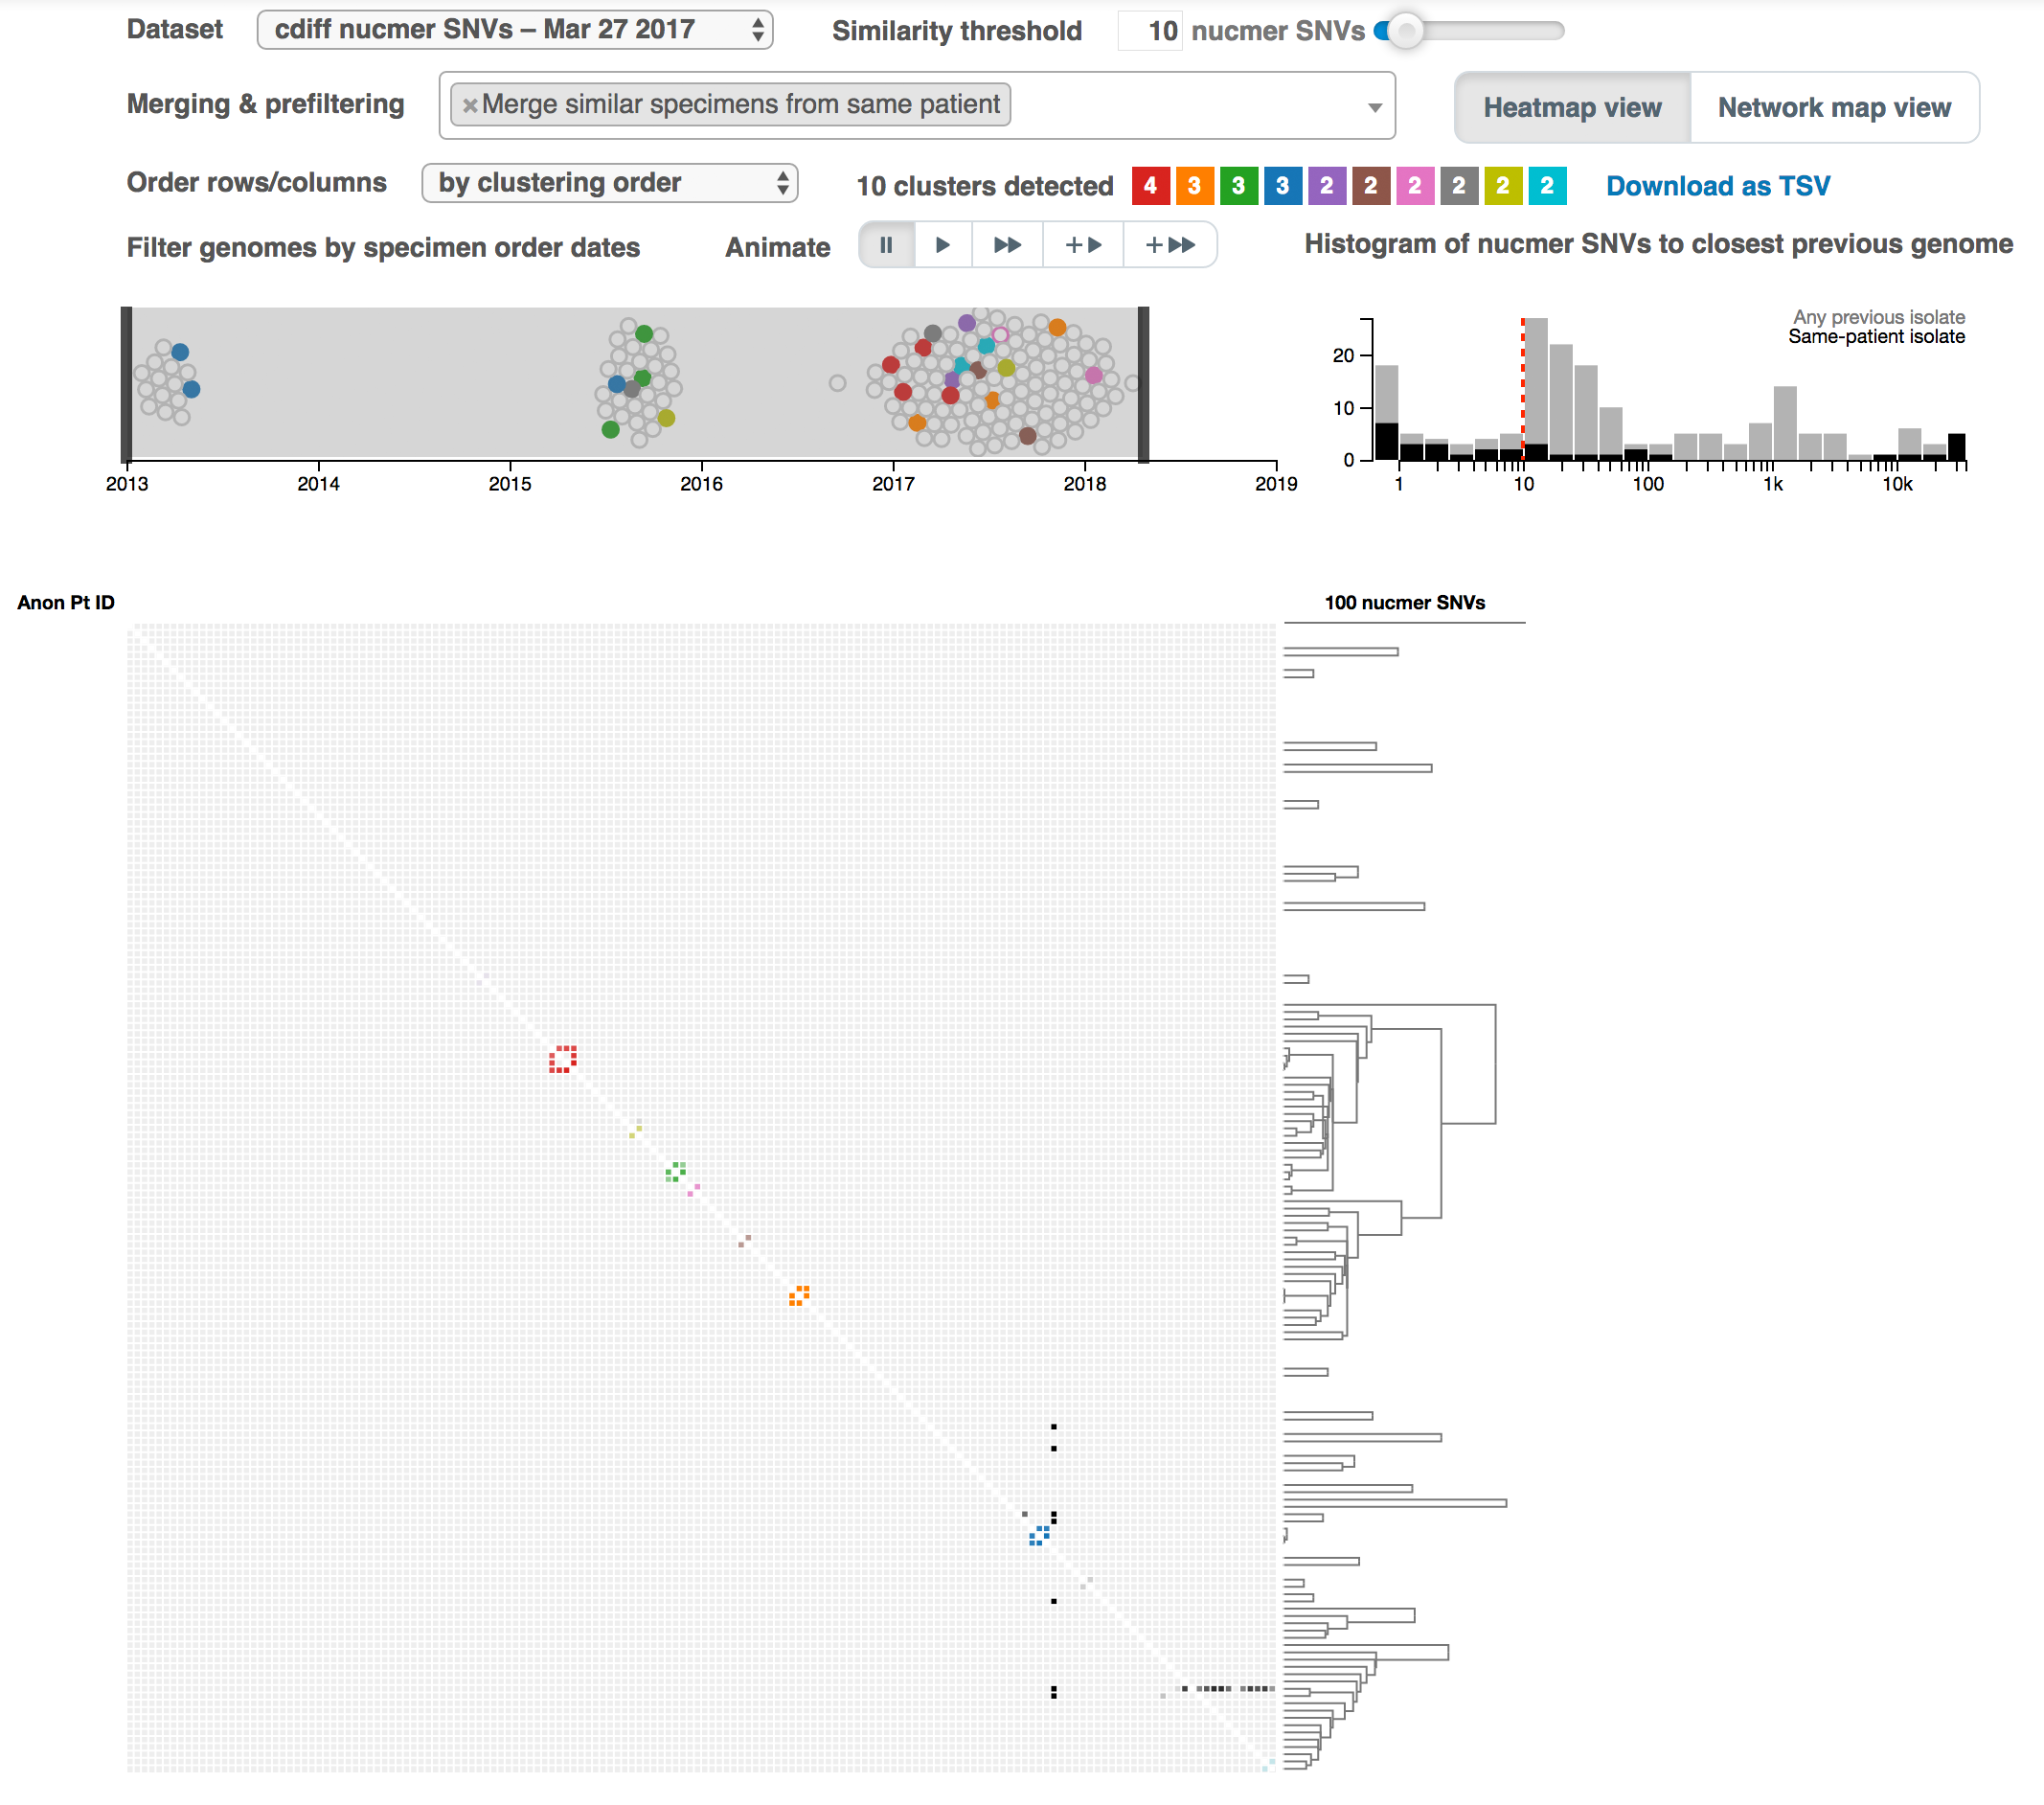
\includegraphics[width=0.8\textwidth]{chap4/pdb-heatmap-cdiff}               
  \fullwidthlabelcaption{fig:pdb_heatmap_cdiff}{\pathogendbviz{} heatmap visualization for all sequenced \emph{C. difficile} isolates over a five-year period}{\textbf{\pathogendbviz{} heatmap visualization for all sequenced \emph{C. difficile} isolates over a five-year period.} All conventions used here are equivalent to Figure \ref{fig:pdb_heatmap_saureus}. Note that dates have again been shifted into the future to reduce the disclosure of potentially identifying information, and we have also censored all sample metadata from this screenshot.}
\end{sidewaysfigure}

We now use \pathogendbviz{} to similarly visualize all sequenced isolates of \emph{C. difficile}. While the Pathogen Surveillance Program has collected all positive \emph{S. aureus} cultures over the past \textasciitilde{}2 years, the surveillance of \emph{C. difficile} has been broader, including sequencing of isolates from pilot periods roughly one year and three years before the start of routine daily collection from all Mount Sinai units \textasciitilde{}1.5 years ago. This is reflected in the trimodal distribution of isolates along the timeline in Figure \ref{fig:pdb_heatmap_cdiff}, where we have included all isolates, not just putative transmissions. We set a similar SNV threshold of 10 SNVs for this longer time period based on the histogram of SNV distances (top right of Figure \ref{fig:pdb_heatmap_cdiff}). Under this threshold, we discover ten small clusters, the largest of which has four patients and with most having only two. Scanning the color of the dots in the timeline indicates that most of the clusters sensibly fall within month-scale intervals, although the yellow-green, gray, and blue clusters are remarkable for spanning the >1 year gaps between the different surveillance periods.

The heatmap visualization at the bottom left of Figure \ref{fig:pdb_heatmap_cdiff} shows the clusters as small groups along the diagonal, and the clustering dendrogram at bottom right shows that some of the clusters separate from each other by distances of \textasciitilde{}20 SNVs.\footnote{Recall the current estimates of the mutation rate for \emph{C. difficile} are around 2-3 SNVs per year; see \textcite{Eyre2013,Price2014,Eyre2012}.} Therefore, there is certainly some interplay between \emph{C. difficile} evolution in the local community and what eventually arrives at Mount Sinai. What is more notable is how most of our isolates are in fact not related across this five year capturing period (the heatmap is mostly blank), which indicates that patient-to-patient transmission is \emph{not} our usual source of \emph{C. difficile} infections and lends support to the more recent hypotheses regarding asymptomatic colonization followed by microbiotic dysregulation.\autocite{Weingarden2015,Bagdasarian2015}

Note that there are some spurious low SNV distances seen in the lower right of the heatmap (unclustered black squares) caused by two low-quality assemblies, which should be re-examined. Low-quality assemblies can appear to have no SNVs if they contain too much redundant sequence, usually caused by a contig that was not merged correctly into the final assembly that prevents subsequences from aligning uniquely. By using single-linkage hierarchical clustering and displaying all intracluster distances, the heatmap can therefore provide some resiliency against errors inadvertently introduced among any of the upstream steps.

\begin{sidewaysfigure}[hp]
  \sidewaysvspace
  \centering
  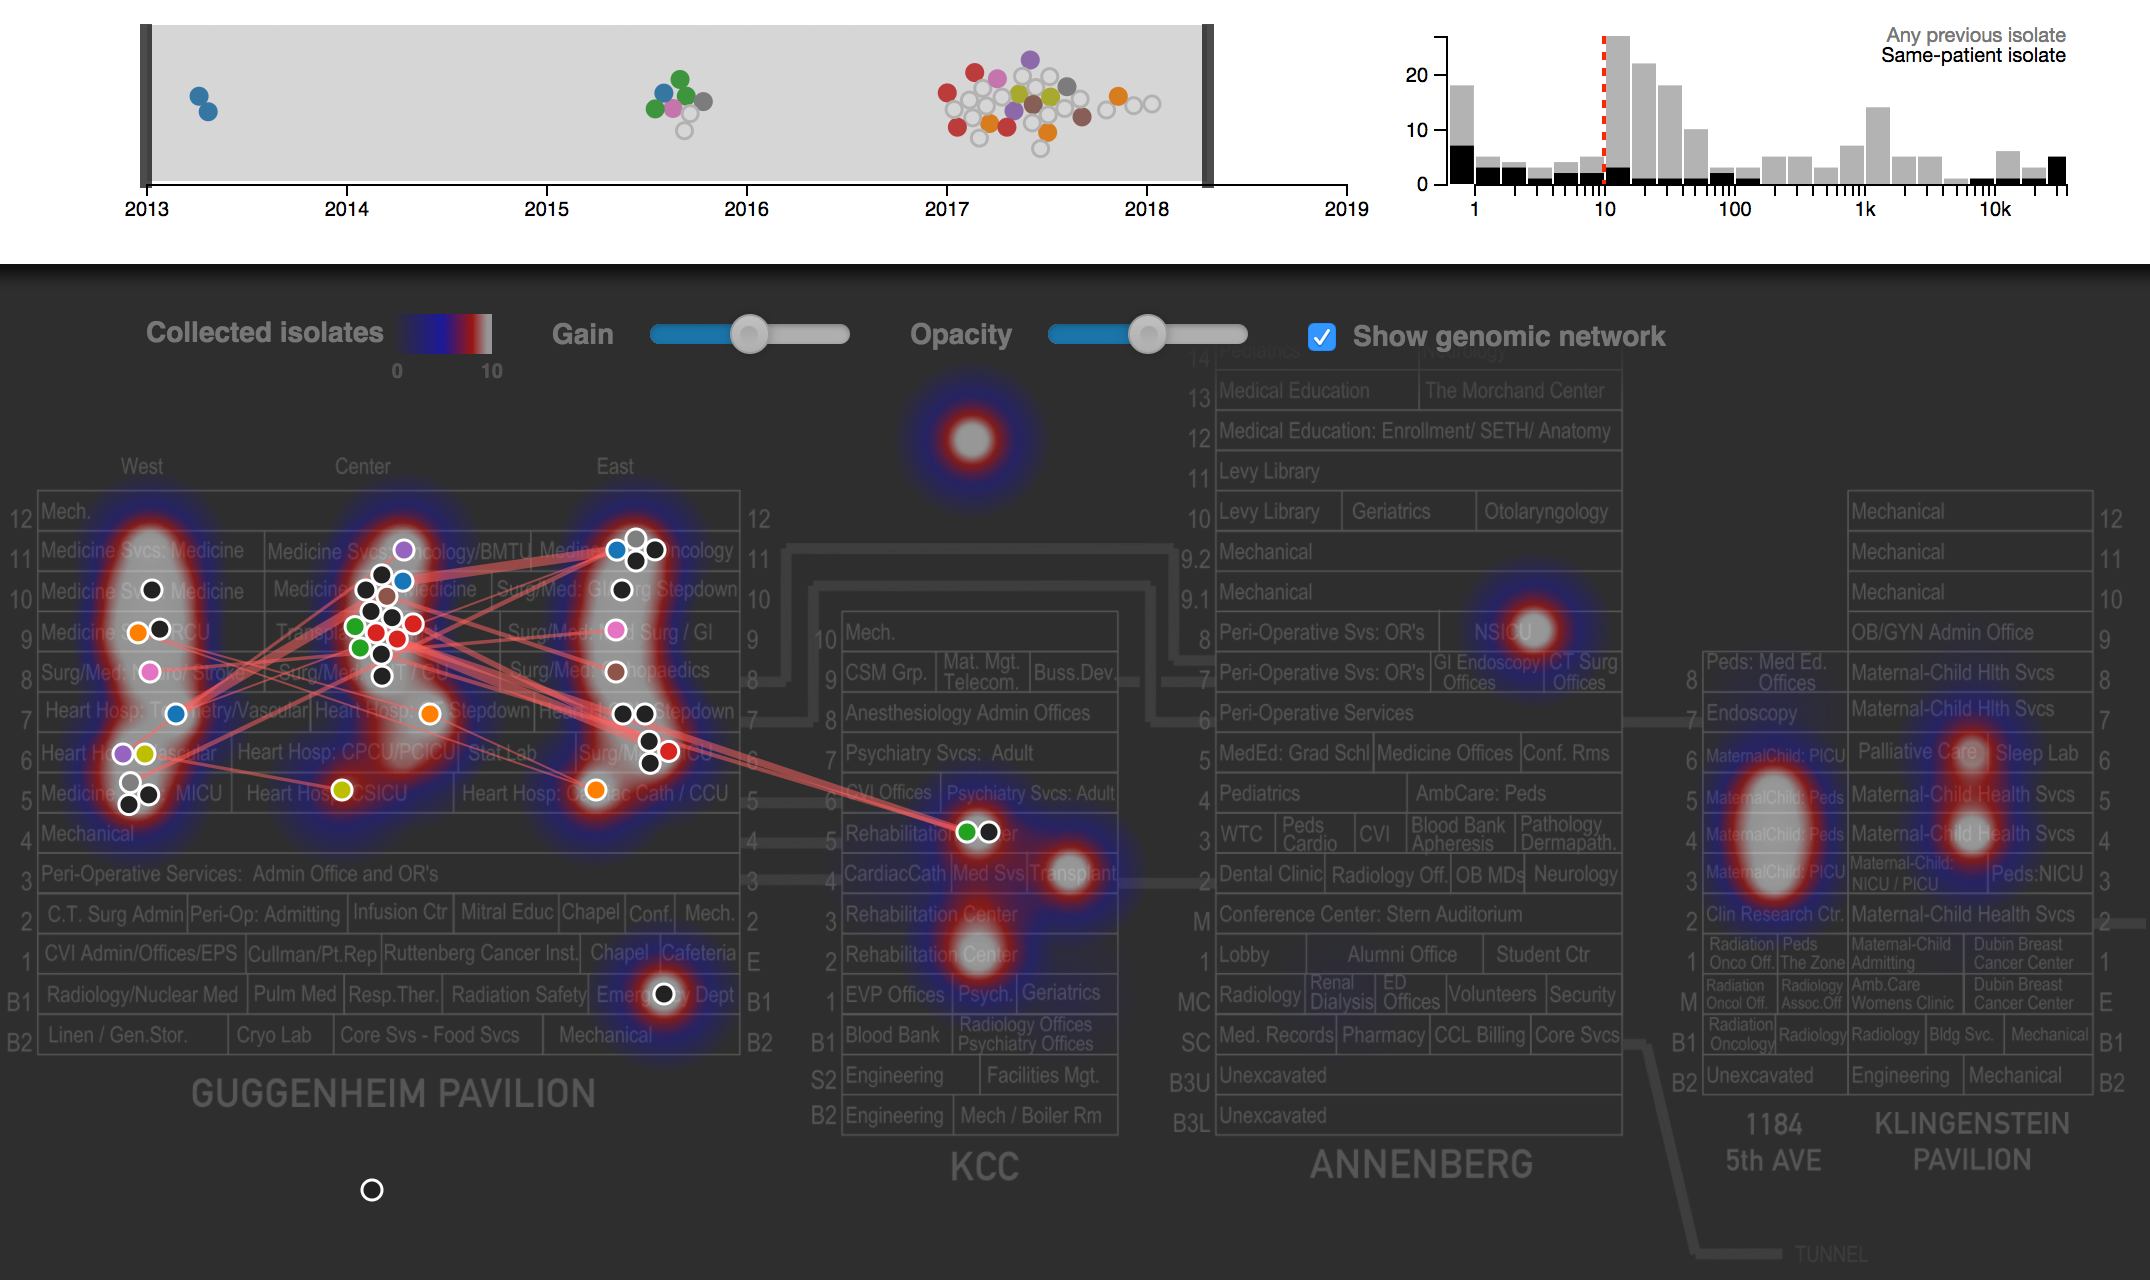
\includegraphics[width=\textwidth]{chap4/pdb-geospatial-cdiff}               
  \fullwidthlabelcaption{fig:pdb_geospatial_cdiff}{\pathogendbviz{} geospatial visualization for NGS-confirmed clusters of \emph{C. difficile} isolates over a five-year period}{\textbf{\pathogendbviz{} geospatial visualization for NGS-confirmed clusters of \emph{C. difficile} isolates over a five-year period.} All conventions used here are equivalent to Figure \ref{fig:pdb_geospatial_saureus}.  Note that dates have been shifted into the future to reduce the disclosure of potentially identifying information.}
\end{sidewaysfigure}

Finally, we can again visualize the spatial relationships among clusters using the network map view in Figure \ref{fig:pdb_geospatial_cdiff}. In this view, which is now focused only on isolates with at least one link to a different-patient isolate, we see that most of the clusters are spread across multiple units (red lines). There are even  NGS-confirmed links between a unit in KCC and the units in Guggenheim. Although considering all the hypothetical reasons for this pattern is beyond the scope of this chapter, our data does suggest that patient-to-patient transmission of \emph{C. difficile} spores is occuring across substantial spatial distances within Mount Sinai, whether due to the movements of patient, staff, or equipment.

\section{Conclusions}

We have developed a new open-source software suite, PathogenDB, that permits semi-automated epidemiological analysis of HAIs based on long-read sequencing and \emph{de novo} assembly of all isolates. We chose a modular design, separating concerns into a LIMS that centralizes storage of the most up-to-date data, a genome assembly and annotation workflow called \pathogendbpipeline, a comparative genomics toolkit called \pathogendbcomparison, and the visualization tool \pathogendbviz. Thus far,we have assembled and annotated 593 genomes, mostly of \emph{S. aureus} and \emph{C. difficile}, using \pathogendbpipeline{}. This part of the analysis, which is the most computationally intensive, can run in 2-3 hours per isolate on a single server (Figure \ref{fig:pdb_benchmark}) and in >70\% of cases can completely finish the genome assembly without human intervention (Table \ref{tab:pathogendb_assemblies}). We can then integrate phylogenetic and epidemiological analyses into a ``live view'' of putative transmissions mapped to hospital locations, using novel interactive heatmap and network map layout visualizations as implemented in \pathogendbviz.

Our software suite was able to genomically characterize one known MRSA outbreak (red cluster in Figure \ref{fig:pdb_heatmap_saureus}) and discover a previously unknown MRSA outbreak (orange cluster in Figures \ref{fig:pdb_heatmap_saureus}-\ref{fig:pdb_geospatial_saureus}). We have likewise used it to characterize the incidence and spatial distribution of patient-to-patient transmission of \emph{C. difficile} across a surveillance period of five years (Figures \ref{fig:pdb_heatmap_cdiff}-\ref{fig:pdb_geospatial_cdiff}). Addtionally, we used earlier versions of our software to characterize two transmissions via solid organ transplant,\autocite{Altman2014,Bashir2017} and pseudo-outbreaks of \emph{B. cepacia} and \emph{S. maltophilia}.\autocite{Pak2015a} The three modules of the PathogenDB suite are freely available on GitHub (see Availability above) and are being prepared for public use in generic computing environments.

\section*{Notes}

\subsection*{Contributions}

Theodore R. Pak (\smallcaps{TRP}), Mitchell Sullivan (\smallcaps{MS}), Oliver Attie (\smallcaps{OA}), Elizabeth Webster (\smallcaps{EW}), Robert Sebra (\smallcaps{RS}), Camille L. Hamula (\smallcaps{CLH}), Gintaras Deikus, (\smallcaps{GD}), Leah C. Newman (\smallcaps{LCN}), Gopi Patel (\smallcaps{GP}), Deena R. Altman (\smallcaps{DRA}), Shirish Huprikar (\smallcaps{SH}), Ali Bashir (\smallcaps{AB}), Andrew Kasarskis (\smallcaps{AK}), and Harm van Bakel (\smallcaps{HVB}) contributed to this chapter. 

\smallcaps{TRP} wrote the first versions of \pathogendbpipeline, \pathogendbcomparison, and \pathogendbviz. \smallcaps{TRP}, \smallcaps{MS}, \smallcaps{OA}, \smallcaps{HVB}, \smallcaps{AB}, and \smallcaps{EW} have contributed code to the current version of \pathogendbpipeline. \smallcaps{TRP}, \smallcaps{MS}, \smallcaps{OA}, \smallcaps{HVB}, and \smallcaps{EW} have contributed code to the current version of \pathogendbcomparison. \smallcaps{TRP} wrote the current version of \pathogendbviz. \smallcaps{HVB} created and maintains the PathogenDB database. \smallcaps{DRA}, \smallcaps{GP}, \smallcaps{HVB}, \smallcaps{AB}, and \smallcaps{CLH} organized collection of samples. \smallcaps{GD}, \smallcaps{LCN}, and \smallcaps{RS} prepared sequencing libraries and performed sequencing. \smallcaps{CLH} performed culturing and drug susceptibility testing. \smallcaps{TRP}, \smallcaps{MS}, \smallcaps{OA}, \smallcaps{RS}, \smallcaps{EW}, \smallcaps{HVB}, and \smallcaps{AB} performed data analysis. \smallcaps{SH}, \smallcaps{GP}, and \smallcaps{AK} provided institutional support and critical feedback on \pathogendbviz. \smallcaps{TRP} created all figures and wrote the first draft of this chapter.

\subsection*{Funding}

Funding was provided by the Icahn Institute for Genomics and Multiscale Biology at Mount Sinai. \smallcaps{TRP} was supported by the Icahn Institute for Genomics and Multiscale Biology at Mount Sinai and NIH/NIAID (U19-AI118610 and F30-AI122673). Research was also supported by the Office of Research Infrastructure of the NIH under award number S10-OD018522. The content is solely the responsibility of the authors and does not necessarily represent the official views of NIH.

\subsection*{Conflict of Interest}

The authors have no conflicts of interest to disclose.

\subsection*{Acknowledgements}

We thank Timothy O’Donnell, Tavi Nathanson, and members of the clinical microbiology laboratory at Mount Sinai for their contributions. This work was supported in part by the resources and expertise of the Department of Scientific Computing at the Icahn School of Medicine at Mount Sinai.
